\documentclass[twoside, 12pt]{article}
\usepackage[utf8]{inputenc}
\usepackage{abstract,lipsum}
\usepackage[english,french]{babel}
\usepackage{geometry}
 \geometry{
 a4paper,
 total={160mm,247mm},
 left=30mm,
 top=30mm,
 asymmetric
 }
\usepackage{eso-pic}
\usepackage{xcolor}
\usepackage{ragged2e}
\usepackage{fancyhdr}
\usepackage[nottoc, notlof, notlot,numbib]{tocbibind}
\usepackage{caption}
\usepackage{subcaption}
\usepackage{hyperref}
\usepackage{booktabs}
\usepackage{amsmath}
\usepackage[]{algorithm2e}
\usepackage{amssymb}
\usepackage{graphicx} % Allows including images
\usepackage{booktabs} % Allows the use of \toprule, \midrule and \bottomrule in tables
\usepackage{float}
\usepackage{appendix}
\usepackage{multirow}
\usepackage{siunitx}

\usepackage[table]{xcolor}
\DeclareCaptionLabelFormat{continued}{#1~#2 (Continued)}
\captionsetup[continuedfloat]{labelformat=continued}
\usepackage{placeins}

\usepackage{listings}
\lstset { %
    language=python, % set backgroundcolor
    basicstyle=\footnotesize,% basic font setting
}

\newcommand{\mycode}{                               % Name after the Language used
    \lstset{
        basicstyle=\ttfamily\small,                 % Code Font Size
        keywordstyle=\color{darkpurple}\bfseries,   % Color Key Word
        stringstyle=\color{darkblue},               % Color String
        identifierstyle=\color{teal},
        commentstyle=\color{darkgreen},             % Color Comment
        morecomment=[s][\color{blue}]{/**}{*/},     % Color Comment
        tabsize=2,                                  % Tab Size
        captionpos=b,                               % Caption Position
        showtabs=false,                             % Show Tabs within Strings
        showspaces=false,                           % Show Spaces Code
        showstringspaces=false,                     % Show Spaces Strings
        stepnumber=1,                               % Line Number Step
        numbers=left,                               % Line Number Position
        numbersep=5pt,                              % Line Number Distance from Code
        numberstyle=\tiny\color{gray},              % Line Number Style
        frame=single,                               % Frame
        rulecolor=\color{black},                    % Frame Color
        xleftmargin=10pt,                            % Left Margin
        backgroundcolor=\color{white},              % Background Color
        breaklines=true,                            % Break Automatic Line
        breakatwhitespace=true,                     % Break Automatic Spaces 
        breakautoindent=false,                      % Break Automatic Indent
        extendedchars=true,                         % 
        inputencoding=latin1,                       % Encoding
        literate=                                   % Including Especial Charects To Write in French
                {é}{{\'{e}}}1
                {è}{{\`{e}}}1
                {ê}{{\^{e}}}1
                {ë}{{\¨{e}}}1
                {É}{{\'{E}}}1
                {Ê}{{\^{E}}}1
                {û}{{\^{u}}}1
                {ù}{{\`{u}}}1
                {ú}{{\'{u}}}1
                {â}{{\^{a}}}1
                {à}{{\`{a}}}1
                {á}{{\'{a}}}1
                {ã}{{\~{a}}}1
                {ä}{{\"{a}}}1
                {Á}{{\'{A}}}1
                {Â}{{\^{A}}}1
                {Ã}{{\~{A}}}1
                {Ä}{{\"{A}}}1
                {ç}{{\c{c}}}1
                {Ç}{{\c{C}}}1
                {õ}{{\~{o}}}1
                {ó}{{\'{o}}}1
                {ô}{{\^{o}}}1
                {ö}{{\"{o}}}1
                {Õ}{{\~{O}}}1
                {Ó}{{\'{O}}}1
                {Ô}{{\^{O}}}1
                {Ö}{{\"{O}}}1
                {î}{{\^{i}}}1
                {Î}{{\^{I}}}1
                {í}{{\'{i}}}1
                {Í}{{\~{Í}}}1
                {ü}{{\"{u}}}1
                {Ü}{{\"{U}}}1
    }
}

\usepackage[alf,bibjustif,abnt-etal-cite=3,abnt-etal-list=0,abnt-repeated-author-omit=yes]{abntex2cite}
\bibliographystyle{abntex2-alf}

\makeatletter
\renewenvironment{titlepage}
 {%
  \if@twocolumn
    \@restonecoltrue\onecolumn
  \else
    \@restonecolfalse\newpage
  \fi
  \thispagestyle{plain}%
 }
 {%
  \if@restonecol
    \twocolumn
  \else
    \newpage
  \fi
 }
\makeatother

\providecommand{\keywords}[1]
{
  \small	
  \textbf{\textit{Keywords---}} #1
}

\newcommand{\source}[1]{\caption*{Source: {#1}} }

%\title{Projet de Recherche (PRe}
\author{Luana DE QUEIROZ GARCIA}
\date{May 2024}

% -----------------------------------------------------------------
% Top and bottom of the pages are set here
% -----------------------------------------------------------------
\pagestyle{fancy}
\fancyhf{}
\fancyhead[CO]{Explainability of high-dimensional prediction models using neural networks}
\fancyhead[CE]{\rightmark}
\cfoot{DE QUEIROZ GARCIA Luana - INRIA Paris \break \color{red} This work is non confidential}
\rfoot{\thepage}

\begin{document}

% -------------------------------------------
% Title Page
% -------------------------------------------

\begin{titlepage}
    \thispagestyle{empty}

    \begin{figure}[h]
    \centering
    \begin{minipage}[b]{0.3\textwidth}
        \raggedright
        % \includegraphics[height=0.55\textwidth]{logo_ENSTA_Paris.jpg} old logo from ENSTA
        
\includegraphics[height=0.45\textwidth]{Images/logos/logo_ensta.png}
    \end{minipage}
    \hfill
    \begin{minipage}[b]{0.3\textwidth}
        \raggedleft
        
\includegraphics[height=0.4\textwidth]{Images/logos/inr_logo_rouge.png}
    \end{minipage}
    \hfill
    \begin{minipage}[b]{0.3\textwidth}
        \raggedleft
        
\includegraphics[height=0.5\textwidth]{Images/logos/logo-IMT.png}
    \end{minipage}
    \end{figure}
    
    \vfill
    
    \centering{\LARGE \textbf{Research Internship (PRe)}} \\
    \hfill\\
    \centering{\large \textbf{Field of Study: Explainable AI}}\\
    \centering{\large \textbf{Scholar Year : 2024-2025}} \\
    \hfill\\
    \vfill
    \centering{\huge \textbf{Explainability of high-dimensional prediction models using neural networks}}
    \vfill
     \color{red} \noindent  \fbox{%
     \parbox{\textwidth}{%
        \centering{\LARGE \textbf{Confidentiality Notice}}\\
        \centering{\normalsize Non-confidential and publishable report}
        }%
    }
    \vfill
    \color{black}
    \large \textbf{Author: DE QUEIROZ GARCIA Luana \hfill Promotion: 2026}\\
    \vspace{5mm}
    \FlushLeft{\normalsize \textbf{ENSTA Paris Tutor: Alexandre CHAPOUTOT}} \\
    \normalsize \textbf{Host Organism Tutor: Jean-Michel Loubes}
    
    \vfill
    \centering{\normalsize \textbf{Internship from 26/05/2025 to 22/08/2025}} \\
    \vspace{1cm}
    \centering{\normalsize \textbf{INRIA Paris}} \\
    \centering{\normalsize \textbf{Address: 48 Rue Barrault, Paris, France}}
\end{titlepage}


% -------------------------------------------
% Blank page (?)
% -------------------------------------------
\section*{}
\vfill
\paragraph{}
\begin{center}
    This page was intentionally left blank.
\end{center}
\vfill

% -------------------------------------------
% Confidentialy Notice
% -------------------------------------------
\newpage

\section*{Confidentialy Notice}
\vfill
\paragraph{}
This present document is not confidential. It can be communicated outside in paper format
or distributed in electronic format.
\vfill

% -------------------------------------------------------------------
% Writing part
% -------------------------------------------------------------------

\selectlanguage{english}

\begin{abstract}
The increasing complexity of machine learning models, particularly deep neural networks for weather forecasting and large language models, has created a critical need for robust Explainable AI (XAI) techniques. These "black box" models operate on high-dimensional data, making it difficult to understand their predictions and trust their outputs. This work evaluates the effectiveness of XAI methods, specifically the Anchors technique, in providing actionable insights across two diverse data domains: tabular data for fairness auditing and high-dimensional meteorological data for weather prediction.

We adopt a two-tiered methodology. First, we apply Anchors to the Folktables dataset to audit a binary income classifier, demonstrating its ability to identify precise, high-precision rules that reveal model vulnerabilities and biases, such as a reliance on sensitive attributes like gender. This provides a granular understanding of discriminatory mechanisms, a crucial step towards targeted bias mitigation. Second, we adapt and extend the Anchors framework for regression tasks to analyze a UNetR++ model trained on the Titan meteorological dataset. Our method successfully pinpoints the most influential spatial regions and variables (e.g., wind patterns, precipitation) for specific forecasts, transforming Anchors into a tool for regional influence analysis and proactive vulnerability mapping for extreme weather events.

Our results show that the Anchors method provides focused, direct, and actionable insights regardless of data complexity. It proves to be a versatile tool not only for diagnosing societal biases in algorithms but also for auditing the physical reasoning of complex forecasting models. This work establishes a foundation for using example-based explainability as a guide for actionable intervention, enhancing trust and providing a pathway for improvement in both technical and societal systems.
\end{abstract} \hspace{10pt}
\keywords{Explainable AI (XAI), Anchors, Model Interpretability, Fairness in Machine Learning, Meteorological Forecasting, High-Dimensional Data, Bias Detection.}

\selectlanguage{french}

\begin{abstract}
La complexité croissante des modèles d'apprentissage automatique, en particulier des réseaux de neurones profonds pour la prévision météorologique et des grands modèles de langage, a créé un besoin critique de techniques robustes d'IA explicable (XAI). Ces modèles « boîte noire » traitent des données à haute dimensionnalité, ce qui rend difficile la compréhension de leurs prédictions et la confiance dans leurs sorties. Ce travail évalue l'efficacité des méthodes XAI, en particulier la technique Anchors, à fournir des insights actionnables dans deux domaines de données divers : les données tabulaires pour l'audit de l'équité et les données météorologiques à haute dimensionnalité pour la prévision du temps.

Nous adoptons une méthodologie à deux niveaux. Premièrement, nous appliquons Anchors au jeu de données Folktables pour auditer un classificateur binaire de revenu, démontrant sa capacité à identifier des règles précises et à haute précision qui révèlent les vulnérabilités et les biais du modèle, tels qu'une dépendance à des attributs sensibles comme le genre. Cela fournit une compréhension granulaire des mécanismes discriminatoires, une étape cruciale vers une atténuation ciblée des biais. Deuxièmement, nous adaptons et étendons le cadre Anchors pour les tâches de régression afin d'analyser un modèle UNetR++ entraîné sur le jeu de données météorologiques Titan. Notre méthode identifie avec succès les régions spatiales et les variables les plus influentes (par exemple, les régimes de vent, les précipitations) pour des prévisions spécifiques, transformant Anchors en un outil d'analyse d'influence régionale et de cartographie proactive de la vulnérabilité pour les événements météorologiques extrêmes.

Nos résultats montrent que la méthode Anchors fournit des insights focalisés, directs et actionnables, indépendamment de la complexité des données. Elle s'avère être un outil polyvalent, non seulement pour diagnostiquer les biais sociétaux dans les algorithmes, mais aussi pour auditer le raisonnement physique de modèles de prévision complexes. Ce travail établit une base pour utiliser l'explicabilité basée sur des exemples comme guide pour une intervention actionable, améliorant la confiance et offrant une voie d'amélioration pour les systèmes techniques et sociétaux.
\end{abstract} \hspace{10pt}
\keywords{IA Explicable (XAI), Anchors, Interprétabilité des modèles, Équité en apprentissage automatique, Prévision météorologique, Données à haute dimensionnalité, Détection de biais.}

\renewcommand{\keywords}[1]
{
  \small	
  \textbf{\textit{Mots clés---}} #1
}

\selectlanguage{english}

\section*{Acknowledgments}
I am deeply grateful to all those who have contributed to the successful completion of this research project during my internship at INRIA Paris and at the Institute of Mathematics of Toulouse (IMT).

I extend my sincere gratitude to my advisors, Laurent Risser, Benoit Rottembourg, and Jean-Michel Loubes, for welcoming me into this internship. I greatly appreciate the opportunity to have learned so much about both fields of fairness, bias correction, explainability, and meteorological prediction. I am especially thankful to Laurent for his close guidance and for his genuine interest in me as an intern from the very beginning.

I would also like to express my special thanks to Laure Raynaud for her supervision at Météo-France and to Corentin Seznec for his valuable support and insights.

Furthermore, I extend my appreciation to my office colleague, Marie Boyer, for her contribution of ideas and stimulating discussions throughout the internship.

This has been a truly special opportunity, and it is an area I intend to pursue in the future.

\newpage
\tableofcontents

\newpage
\listoffigures

\fancyhead[CE]{\leftmark}
\section{Introduction}

The use of machine learning, particularly through deep neural network models, has recently revitalized various fields of mathematical engineering. Notably, the domain of weather forecasting has seen the emergence of new players from the world of machine learning \cite{graph-cast-remi} \cite{weather-forecasting-bi}, whose predictive model quality approaches that of traditional weather forecasting models. However, models resulting from this work, such as GraphCast, are highly complex and handle very high-dimensional data. As a result, it is currently very difficult to assess the criteria on which they base their predictions, which may limit confidence in their forecasts. These models can be likened to Large Language Models (LLMs), sharing many architectural similarities and exhibiting comparable complexities.  

As part of this internship, we will evaluate the relevance of eXplainable AI (XAI) methods for high-dimensional AI predictions. To systematically assess the robustness and limitations of these techniques, we adopt a two-tiered approach. First, we apply XAI methods to a simpler, well-understood domain: supervised classification on tabular data (using the Folktables dataset). This allows us to benchmark the methods' ability to identify biases and vulnerabilities, such as reliance on sensitive attributes like gender. Second, we leverage these insights to tackle the core challenge: applying and adapting XAI techniques to complex, high-dimensional meteorological data from the MeteoNet project \cite{meteo-net}. The ultimate goal is to determine if these methods can uncover the learned concepts, mechanisms, and potential failure points within complex deep learning models used for weather prediction.

The first stage of the internship involved familiarizing ourselves with different forecasting models, understanding their underlying mechanisms, and assessing the quality of their predictions, as well as applying fairness metrics to tabular data to detect bias. Following an approach similar to \cite{guide-xai-bommer}, we then evaluated various explainability methods on both data types, generalizing the methodology (\cite{guide-xai-bommer}). We developed methods based on concept and anchor creation to assess their stability and determine whether we can uncover learned concepts or mechanisms within the network that help better understand its functioning.

The internship will take place at INRIA Paris in collaboration with the Institute of Mathematics of Toulouse (IMT), under the supervision of Jean-Michel Loubes (INRIA), Benoit Rottembourg (INRIA), and Laurent Risser (ANITI).

\subsection{Objectives and division of the report}

The primary objective of this research is to conduct a comprehensive analysis of explainable AI methods (XAI) for complex data, developed at INRIA Paris, and evaluate how to use these different methods across diverse data types. A core aim is to test their ability to reveal vulnerabilities, such as spurious correlations or reliance on sensitive features, in both simple and complex models. Specific objectives include:

\begin{itemize}
    \item To analyse model fairness using standard metrics.
    \item To apply and evaluate Anchors XAI on tabular data to audit model fairness and identify biases.
    \item To understand the structure and challenges of meteorological and image data.
    \item To understand the differences between Anchors-based explanations applied on classification and regression.
    \item To develop and adapt methods for applying XAI techniques to high-dimensional meteorological data.
\end{itemize}

This report is structured into the following sections to systematically address the research objectives:

\begin{itemize}
    \item \textbf{Introduction}: Provides background on the challenges of interpretability in high-dimensional models like weather forecasting and introduces the need for explainable AI (XAI) methods to enhance trust and understanding. It outlines the strategy of using tabular data as a controlled testbed before tackling meteorological complexity.
    \item \textbf{Literature Review}: Surveys existing XAI techniques (e.g., concept-based explanations, anchors, attention mechanisms) and their applications in climate science and fairness auditing.
    \item \textbf{Methodology}: Describes the datasets (Titan and Folktables), models (e.g., deep neural networks, classical machine learning algorithms), and XAI techniques tested (e.g., SHAP, Anchors, and gradient-based approaches) for both data domains.
    \item \textbf{Results}: Presents the findings from the research, including the effectiveness of XAI in identifying bias in tabular data and the outputs, challenges, and initial results of applying XAI to meteorological models.
    \item \textbf{Discussion}: Interprets the results, discussing the transferability of insights from tabular to complex data, the implications for model trustworthiness, and the comparative strengths of different XAI methods.
    \item \textbf{Conclusion}: Summarizes the key findings on the utility of XAI for uncovering model vulnerabilities, emphasizes the importance of the study, and provides recommendations for future research in applying XAI to complex domains.
\end{itemize}
\section{Literature Review}
This review situates our work at the intersection of explainable AI (XAI) for fairness auditing and the application of advanced AI in meteorological science. We first explore the XAI methodologies that form the basis of our analytical approach. We then survey the state of AI-driven weather forecasting, focusing on the data and model architectures relevant to our study.

\subsection{Foundations of Explainable AI and Fairness}

Our research into fairness auditing is primarily based on the Anchors technique \cite{anchors-ribeiro}. While SHAP \cite{shap-lundberg} is the prevalent model-agnostic explanation method, we chose to focus on Anchors due to its novel formulation of high-precision, "if-then" rules and its under-explored potential. A key differentiator is its coverage metric, which quantifies the applicability of a local explanation to other instances in the dataset, providing a direct measure of a decision rule's generalizability.

This exploration of XAI methods is applied to identify unfairness in models trained on demographic data. The Folktables dataset \cite{folktables-ding} provides a modern, well-structured benchmark for this task, moving beyond the limitations of older standards like UCI Adult. Furthermore, the term "anchor" appears in a distinct yet conceptually relevant context in data assimilation.

\subsection{AI-Driven Weather Forecasting: Data and Models}

The field of numerical weather prediction (NWP) is being revolutionized by AI models that offer unprecedented speed and competitive accuracy. Foundational studies like \cite{weather-forecasting-bi} and \cite{graph-cast-remi} demonstrate how deep learning architectures can outperform or complement traditional physics-based NWP systems, such as the operational integrated forecasting system (IFS) from the European Centre for Medium-Range Weather Forecasts (ECMWF).

Our work is built upon the data produced by these traditional systems. We utilize high-resolution outputs from the AROME model, a limited-area forecasting system, and the global ARPÈGE model \cite{arpege}. Understanding the generation and synergy of this data is crucial. Research such as \cite{gan-arome-brochet} explores emulating AROME outputs with generative models, while \cite{arome-tc-unet-raynaud} successfully applies convolutional architectures like U-Net to specific prediction tasks, such as identifying tropical cyclone structures, directly from AROME forecasts.

For our core model architecture, we focus on the UNETR++ \cite{unetrpp}. This model represents the state of the art in segmentation tasks, particularly in medical imaging, by combining the precise localization of a U-Net with the powerful representational capacity of a Vision Transformer (ViT). Its design is exceptionally well-suited for processing the high-dimensional, spatio-temporal data inherent in meteorological fields, making it a prime candidate for advancing data-driven weather prediction. The guide provided by \cite{guide-xai-bommer} offers a framework for evaluating XAI methods in climate science, ensuring our approach is grounded in domain-specific needs.

\subsection{Explainability for Complex Models: From LLMs to Meteorology}
The challenge of explaining complex, high-dimensional models is a pervasive issue across modern AI, extending far beyond our specific application to include Large Language Models (LLMs) and other deep learning systems. Our methodology is informed by the growing body of work aimed at peeling back the layers of these "black box" models. Applying eXplainable AI (XAI) techniques to such intricate systems, however, presents significant hurdles in selecting appropriate methods and evaluation metrics.

To navigate this complexity, frameworks like the one provided by \cite{guide-xai-bommer} are essential. Focused on climate science, their work offers a crucial discussion on the application of XAI and proposes metrics for their evaluation. This guide highlights and assesses various techniques, including powerful gradient-based methods such as SmoothGrad \cite{smooth-grad-smilkov} and Integrated Gradients \cite{integrated-grad-sundararajan}.

\begin{itemize}
    \item Integrated Gradients attributes a model's prediction to its input features by integrating the gradients along a straight path from a baseline (e.g., a black image) to the actual input. It is renowned for satisfying axiomatic properties like completeness, ensuring the attributions sum to the difference in the model's output between the input and the baseline.
    \item SmoothGrad tackles the visual noise often found in saliency maps by averaging multiple gradient maps computed on inputs with added Gaussian noise. This technique helps highlight the features the model robustly considers important, rather than artifacts resulting from infinitesimal input variations.
\end{itemize}

While these gradient-based methods are a cornerstone of the XAI landscape, our exploration was driven by the potential of a different path, inspired by a conceptual metaphor from numerical weather prediction itself. The work on variational bias correction (VarBC) \cite{varBC-francis} utilizes trusted "anchor observations" to correct for systematic biases in satellite data assimilation. This concept of using a reliable reference to ensure correctness powerfully resonates with the goal of XAI: to "anchor" model explanations in unbiased, factual reasoning and identify decision-making vulnerabilities.

This metaphor directly motivated our focus on the Anchors technique \cite{anchors-ribeiro}. Our conviction to explore this less-traveled path was further strengthened by its successful adaptation to other complex domains. The work by \cite{anchors-sea-of-words-lopardo} provides a critical proof-of-concept, offering an in-depth analysis of Anchors for text data. Their research demonstrates the method's viability for generating interpretable, high-precision rules even within the complex, discrete feature space of language. This successful application on a fundamentally different data type strongly justifies our own investigation into adapting Anchors for the complex, spatial-temporal domain of meteorological imagery.


\section{Methodology}
The initial phase of the internship involved familiarizing ourselves with the datasets we intended to explore.
Throughout the internship, we conducted two projects in parallel: one utilizing the Folktables dataset \cite{folktables} and the other utilizing the Titan dataset \cite{titandataset}. The first project focused on auditing fairness and bias in machine learning models by applying classical XAI methods to tabular data. The second project focused on weather prediction and the adaptation of these XAI methods for complex, high-dimensional data.

This parallel approach served a strategic purpose: to first explore the capability of methods like Anchors to explain individual predictions and reveal model bias on a simpler, more interpretable tabular dataset. The insights gained from this controlled environment were then leveraged to guide our efforts in tracking vulnerable areas and adapting XAI techniques for the multi-dimensional domain of meteorological data.



\subsection{Anchors Method}
\label{sec:anchors-formalization}
It's important to make clear how the method works and the precision and coverage measures for the followings sub-sections.

Following Ribeiro's formalization of the Anchors method \cite{anchors-ribeiro}, we consider a binary classifier $f : \mathcal{X} \rightarrow \{0, 1\}$. For a given instance $x$, the objective is to find a predicate $A$ that explains the prediction $f(x)$ by identifying a minimal set of decisive features.

A predicate $A$ is deemed a valid anchor if it meets a precision threshold, meaning it guarantees the model's output is consistent under local perturbation. Precision is formally defined as:
\begin{equation}
\text{prec}(A) = \mathbb{E}_{D(z|A)} [\mathbf{1}_{f(x) = f(z)}]
\label{eq:prec-anchors}
\end{equation}
where $D(\cdot|A)$ is the conditional distribution of inputs satisfying $A$. The anchor condition is satisfied with high confidence if $P(\text{prec}(A) \geq \tau) \geq 1 - \delta$.

It can be remarked that several sets of conditions can be considered as anchors. To select the most impactful and parsimonious explanation for end-users, the method introduces a coverage measure. The coverage of $A$ is defined as the probability that the predicate holds under the data distribution:
\begin{equation}
\text{cov}(A) = \mathbb{E}_{D(z)} [A(z)]
\label{eq:cov-anchors}
\end{equation}

For a given data distribution $D$, parameters $\tau$ and $\delta$, the optimal anchor is the one with maximum coverage subject to the precision constraint:
\begin{equation}
\arg \max_{A} {\text{cov}(A) \mid P(\text{prec}(A) \geq \tau) \geq 1 - \delta }
\label{eq:max-cov-anchors}
\end{equation}

%%%%%%%%%%%%%%%%%%%%%%%%%%%%%%%%%%%%%%%%%%%%%%%%%%%%%%%%%%%%%%%%%%%%%%%%%%%%%%%%%%%%%%%%%%%%%%%%%%%%%%%%%%%%%%%%%%%%%%%
%%%%%%%%%%%%%%%%%%%%%%%%%%%%%%%%%%%%%%%%%%%%%%% FOLKTABLES  %%%%%%%%%%%%%%%%%%%%%%%%%%%%%%%%%%%%%%%%%%%%%%%%%%%%%%%%%%%
%%%%%%%%%%%%%%%%%%%%%%%%%%%%%%%%%%%%%%%%%%%%%%%%%%%%%%%%%%%%%%%%%%%%%%%%%%%%%%%%%%%%%%%%%%%%%%%%%%%%%%%%%%%%%%%%%%%%%%%

\subsection{Tabular Data}
In this initial work done with Benoît and Jean-Michel we used the Folktables dataset \cite{folktables-ding} to apply the Anchors XAI method and try to identify new ways to detect unfairness related to sensitive variables.

The idea here was to explore Anchors, a method that is under-explored in comparison to SHAP. The Anchors method can be interesting for detecting the features taken into account in the decision-making process that maintain the result for a given individual in the dataset. As a perturbation-based method, it replicates the individual locally and verifies which features are responsible for maintaining the model's prediction.

In the case of the Folktables dataset, we wanted to investigate the \textit{SEX} feature as the sensitive variable, to see if the Anchors method could identify it as a decisive feature in the model's prediction.

\subsubsection{The Folktables Dataset}
The Folktables dataset, used in this part of the study, was derived from the 2018 Census of the United States of America (USA). For manipulating this dataset we used the Python library \cite{folktables}, which provides modules for data extraction tailored to specific prediction tasks. The prediction target we used was ACSIncome, meaning the machine learning model was designed to predict an individual's income bracket. The library defines True predictions for those who receive more than \$50,000 and False for those who receive less.

The variables of the dataset are described in Table \ref{tab:folktables-variables}, and their range of values can be consulted in the documentation \cite{folktables-ding}.

\begin{table}[h]
\centering
\caption{Folktables Dataset Features}
\label{tab:folktables-variables}
\begin{tabular}{lll}
\hline
\textbf{Feature code} & \textbf{Description} \\
\hline
AGEP & Age \\
COW & Class of Worker \\
SCHL & Educational Attainment \\
MAR & Marital Status \\
OCCP & Occupation \\
POBP & Place of Birth \\
RELP & Relationship \\
WKHP & Usual Hours Worked Per Week past 12 Months \\
SEX & Sex \\
RAC1P & Recoded detailed race code \\
\hline
\end{tabular}
\end{table}

\subsubsection{Training Data}
For our analysis, we used data covering the entire United States, as well as data from three of the most populous states: California, Texas, and New York. Each subset of data was trained using four widely adopted machine learning algorithms:

\begin{itemize}
	\item XGBoost (eXtreme Gradient Boosting) – A highly efficient and scalable implementation of gradient boosting, known for its performance in structured data tasks. We leveraged its ability to handle missing values and feature importance estimation.
	
	\item Logistic Regression – A classical linear model for binary and multiclass classification. Despite its simplicity, it served as a strong baseline, particularly for interpreting feature coefficients.
	
	\item Hist Gradient Boosting (Skrub's Scikit-learn implementation) – A fast and memory-efficient gradient-boosting variant that bins input features, making it suitable for large datasets while maintaining competitive accuracy.
	
	\item Simple Neural Network – A feedforward neural network with a limited number of layers to assess whether deeper architectures could capture nonlinear patterns beyond what tree-based models achieved.
\end{itemize}


The algorithms were used for classification tasks to predict whether income was higher (True) or lower (False) than \$50,000.

\subsubsection{Fairness Metrics}
After training the models, we evaluated their performance using accuracy and fairness metrics as explained below:

\begin{itemize}
	\item \textbf{Accuracy}: The proportion of correct predictions (both true positives and true negatives) among all predictions.

	\item \textbf{Disparate Impact (DI)}: Measures the ratio between the proportion of positive outcomes for the protected group (women) versus the privileged group (men). Values close to 1 indicate fairness, while values below 1 suggest bias against the protected group.

	\item \textbf{Equality of Odds}: Examines whether both groups have equal true positive rates and equal false positive rates. Values closer to 1 indicate better fairness.

	\item \textbf{Sufficiency}: Assesses whether the probability of the true outcome is the same across groups given the predicted outcome. Values closer to 1 indicate better fairness.
\end{itemize}

We can see on Table \ref{tab:folktables-results} the results comparing the four models in the three states.

Each model was trained on the training data of the state (indicated in the second column), and the fairness metrics were calculated by comparing them to the test data of the state or the full data of the USA (indicated in the third column) to provide both a local and global comparison.

\begin{table}[h]
\centering
\caption{Model Performance Comparison Across States (Accuracy and Fairness Metrics)}
\label{tab:folktables-results}
\resizebox{\textwidth}{!}
{
\begin{tabular}{llcccccc}
\toprule
\textbf{Model} & \textbf{Training} & \textbf{Testing} & \textbf{Accuracy} & \textbf{Disparate Impact} & \textbf{Equality of Odds} & \textbf{Sufficiency} \\
\midrule
\rowcolor{gray!10}
\multirow{6}{*}{Logistic Regression} 
& \multirow{2}{*}{CA} & CA & 0.56 & 0.67 & 0.84 & 0.95 \\
& & USA & 0.52 & 0.66 & 0.88 & 0.86 \\
\cmidrule(lr){2-7}
& \multirow{2}{*}{TX} & TX & 0.52 & 0.46 & 0.65 & 0.90 \\
& & USA & 0.51 & 0.46 & 0.67 & 0.95 \\
\cmidrule(lr){2-7}
& \multirow{2}{*}{NY} & NY & 0.51 & 0.66 & 0.82 & 0.93 \\
& & USA & 0.52 & 0.64 & 0.86 & 0.88 \\
\midrule

\rowcolor{gray!10}
\multirow{6}{*}{XGBoost} 
& \multirow{2}{*}{CA} & CA & 0.64 & 0.72 & 0.91 & 0.96 \\
& & USA & 0.58 & 0.67 & 0.92 & 0.90 \\
\cmidrule(lr){2-7}
& \multirow{2}{*}{TX} & TX & 0.60 & 0.58 & 0.83 & 0.93 \\
& & USA & 0.58 & 0.58 & 0.85 & 0.95 \\
\cmidrule(lr){2-7}
& \multirow{2}{*}{NY} & NY & 0.61 & 0.75 & 0.92 & 0.96 \\
& & USA & 0.57 & 0.67 & 0.92 & 0.90 \\
\midrule

\rowcolor{gray!10}
\multirow{6}{*}{HistGradientBoosting} 
& \multirow{2}{*}{CA} & CA & 0.63 & 0.71 & 0.90 & 0.94 \\
& & USA & 0.58 & 0.67 & 0.92 & 0.90 \\
\cmidrule(lr){2-7}
& \multirow{2}{*}{TX} & TX & 0.61 & 0.54 & 0.78 & 0.96 \\
& & USA & 0.58 & 0.56 & 0.83 & 0.97 \\
\cmidrule(lr){2-7}
& \multirow{2}{*}{NY} & NY & 0.60 & 0.68 & 0.89 & 0.97 \\
& & USA & 0.58 & 0.64 & 0.90 & 0.91 \\
\midrule

\rowcolor{gray!10}
\multirow{6}{*}{Neural Network} 
& \multirow{2}{*}{CA} & CA & 0.52 & 0.88 & 1.03 & 0.85 \\
& & USA & 0.46 & 0.65 & 0.86 & 0.86 \\
\cmidrule(lr){2-7}
& \multirow{2}{*}{TX} & TX & 0.50 & 0.61 & 0.87 & 0.94 \\
& & USA & 0.49 & 0.77 & 0.96 & 0.81 \\
\cmidrule(lr){2-7}
& \multirow{2}{*}{NY} & NY & 0.51 & 0.76 & 0.93 & 0.92 \\
& & USA & 0.48 & 0.66 & 0.88 & 0.87 \\
\bottomrule
\end{tabular}%
}
\end{table}

As the results with the most contrast are shown for the state of Texas, we will focus on these results for the discussion in the report, but the results for California and New York will be in the Appendix (Section \ref{ap:Opt}).

In Figures \ref{fig:roc_tx}, \ref{fig:roc_ca}, and \ref{fig:roc_ny}, we can see the ROC curves of the models applied to the Texas, California, and New York subsets of the data, respectively.

\begin{figure}[h]
    \centering
    \begin{subfigure}[b]{0.48\textwidth}
        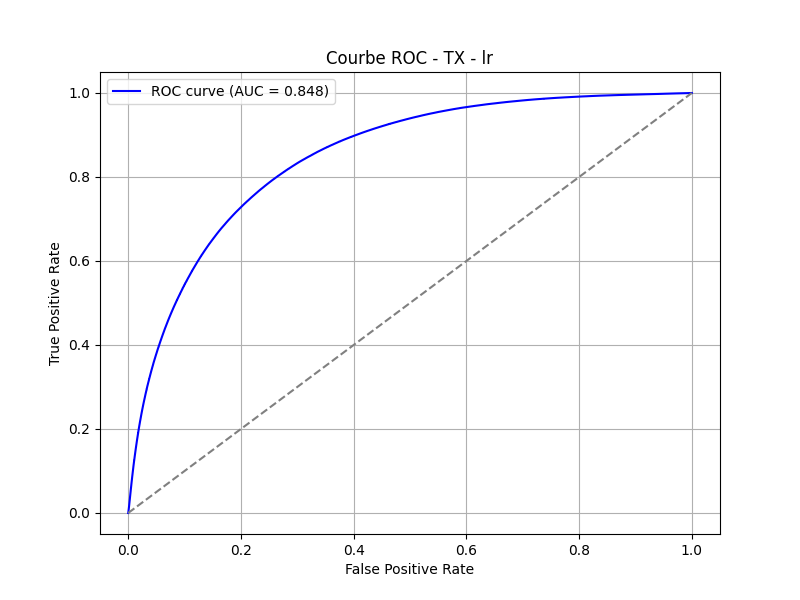
\includegraphics[width=\textwidth]{Images/curve_roc_folktables/roc_curve_TX_lr.png}
        \caption{Curve ROC (AUC = 0.848): model = Logistic Regression}
        \label{fig:TX_lr}
    \end{subfigure}
    \hfill
    \begin{subfigure}[b]{0.48\textwidth}
        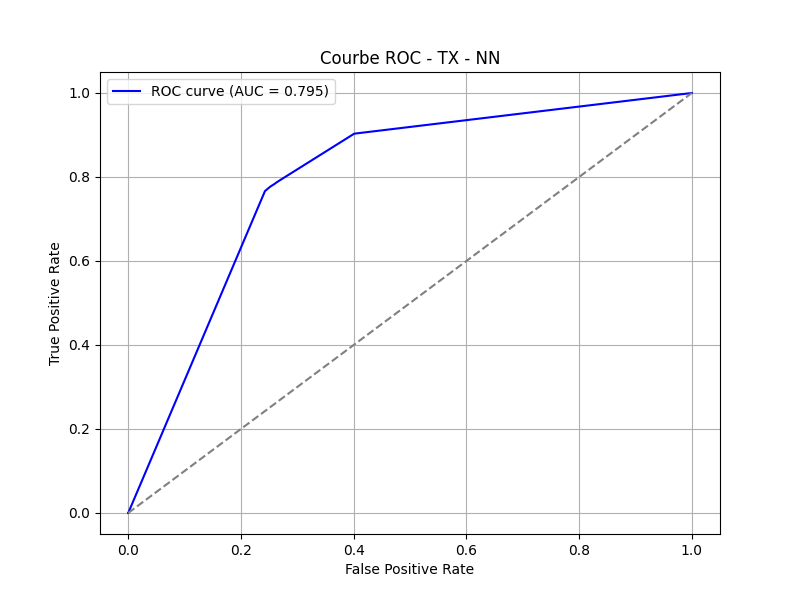
\includegraphics[width=\textwidth]{Images/curve_roc_folktables/roc_curve_TX_NN.png}
        \caption{Curve ROC (AUC = 0.795): model = Neural Network}
        \label{fig:TX_nn}
    \end{subfigure}

    \begin{subfigure}[b]{0.48\textwidth}
        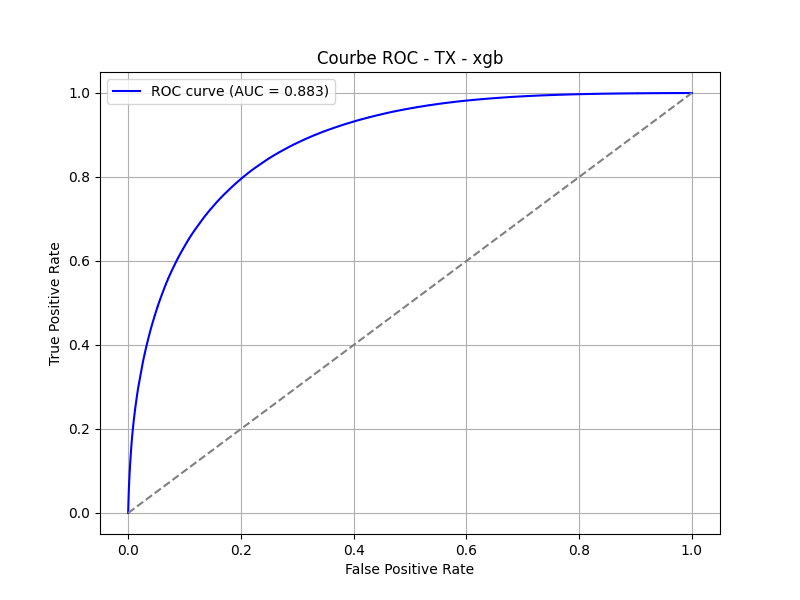
\includegraphics[width=\textwidth]{Images/curve_roc_folktables/roc_curve_TX_xgb.png}
        \caption{Curve ROC (AUC = 0.883): model = XGBoost}
        \label{fig:TX_xgb}
    \end{subfigure}
    \hfill
    \begin{subfigure}[b]{0.48\textwidth}
        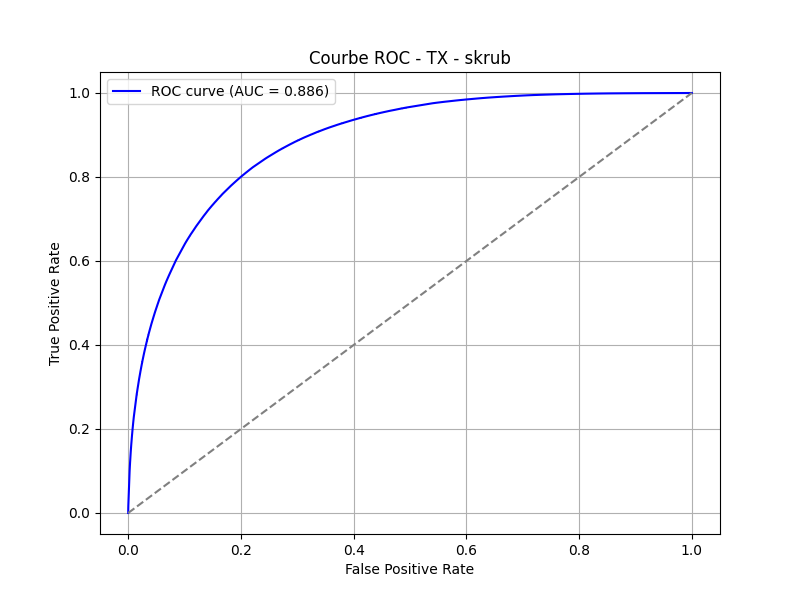
\includegraphics[width=\textwidth]{Images/curve_roc_folktables/roc_curve_TX_skrub.png}
        \caption{Curve ROC (AUC = 0.886): model = HistGradientBoosting}
        \label{fig:TX_skrub}
    \end{subfigure}
    \caption{Comparison of the models trained on the sub dataset of the Texas state}
    \label{fig:roc_tx}
\end{figure}

First, we can see the difference in performances between the models.
In the ROC curve graphics \ref{fig:roc_tx}, \ref{fig:roc_ca}, and \ref{fig:roc_ny}, we can see how XGBoost and HistGradientBoosting outperform the Neural Network, and how Logistic Regression remains average but still does not surpass the others.
Also note that the models with higher accuracy (fourth column) in Table \ref{tab:folktables-results} are XGBoost and HistGradientBoosting.

Second, we can now analyse the fairness metrics in columns five, six, and seven.
It is important to note that the fairness threshold for these metrics, as established by \cite{di-besse}, is 0.8. Values above 0.8 (and closer to 1) are generally considered to indicate fair predictions, while values below this threshold suggest varying degrees of unfairness.
Note that the Equality of Odds and Sufficiency metrics reach higher levels, all of them above 0.8. However, when looking at Disparate Impact (DI), we see a discrepancy from the reference values, with them staying on average 2 percentage points lower.
We interpret this low DI as indicating a discrepancy between women and men who receive more than \$50,000, showing a disadvantage for women in this case.

\subsubsection{Applying XAI Methods}
\label{met:fairness-xai}

After a short analysis of the DI metric for XGBoost and HistGradientBoosting, it is clear that there is a proven bias in the model's prediction. But knowing there is a bias is not enough, so we started using two XAI methods to try to find more information about the bias and try to identify a profile of the individuals who are being discriminated against by the model.

We employed the Anchors method \cite{anchors-ribeiro} to generate and export explanations, aiming to identify the features that were most decisive for the model's predictions.
For the sake of comparison, we also generated and exported the SHAP values of the subsets for further analysis.

We will refer to a \textbf{gendered anchor} when the generated Anchors explanation contains 'SEX' in its list of features, which is the sensitive variable we are analysing. In a similar way, we will refer to \textbf{gendered SHAP values} when the generated SHAP explanation contains 'SEX' at the top of the feature ranking.

\begin{figure}[h]
    \centering
    \begin{subfigure}[b]{0.9\textwidth}
        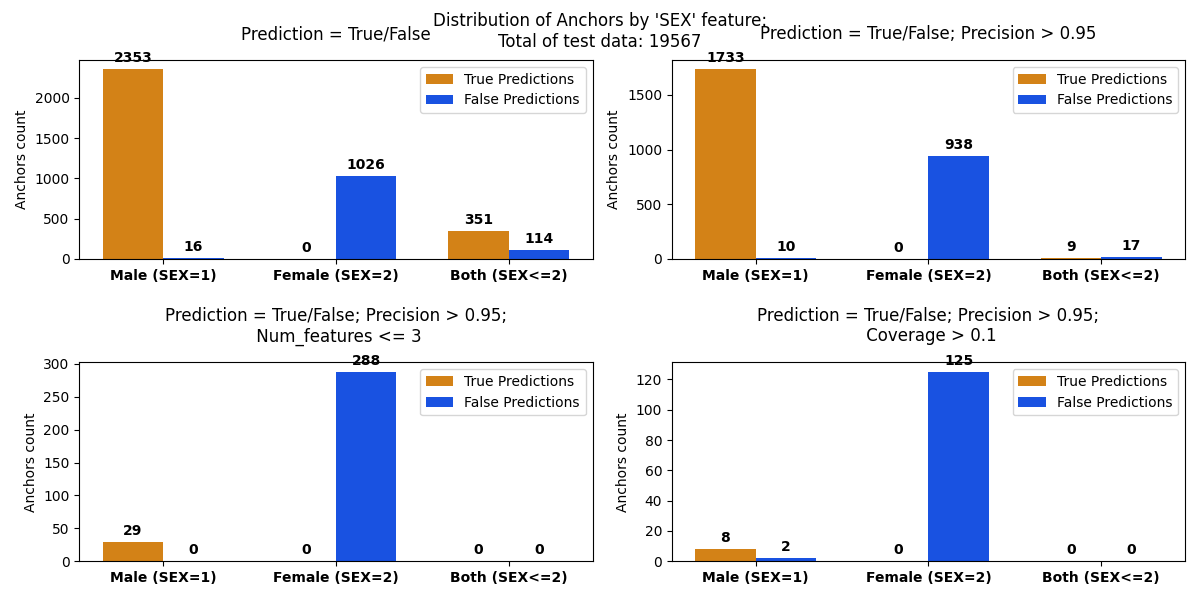
\includegraphics[width=\textwidth]{Images/distribution_folktables/pca_xg_ca_anchors.png}
        \caption{Model: XGBoost, XAI method: Anchors}
        \label{fig:distr_xg_ca_anchors}
    \end{subfigure}
    \hfill
    \begin{subfigure}[b]{0.9\textwidth}
        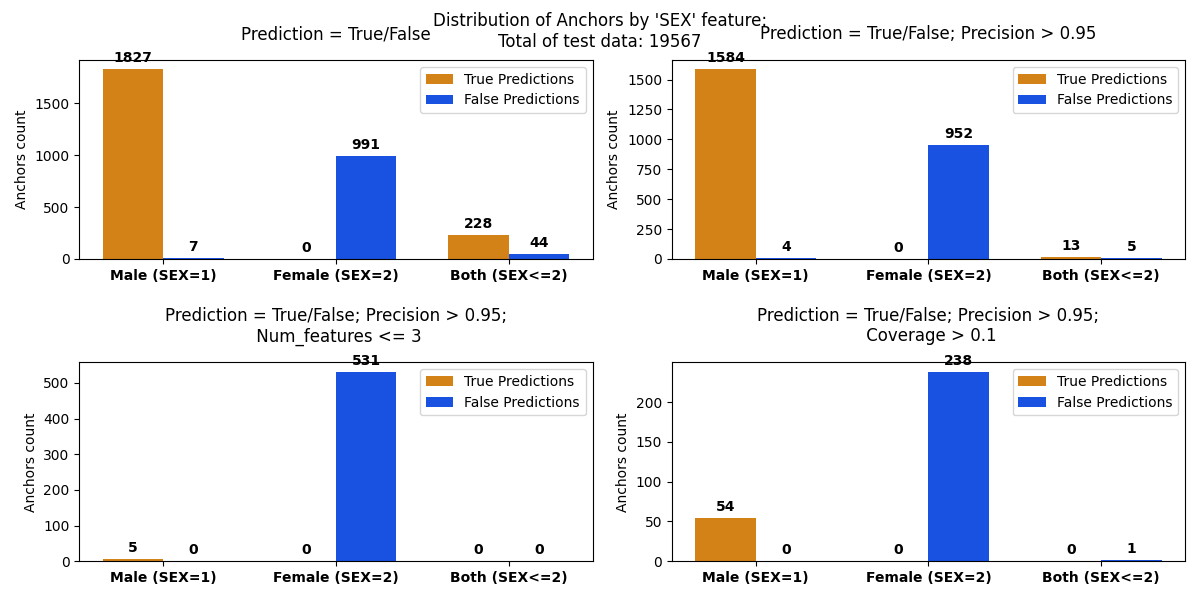
\includegraphics[width=\textwidth]{Images/distribution_folktables/pca_skrub_ca_anchors.png}
        \caption{Model: HistGradientBoosting, XAI method: Anchors}
        \label{fig:distr_skrub_ca_anchors}
    \end{subfigure}
    \caption{Comparison of the gendered explanations between True and False predictions in the California state (Part 1)}
 \end{figure}

\begin{figure}[h]
    \ContinuedFloat
    \begin{subfigure}[b]{0.9\textwidth}
        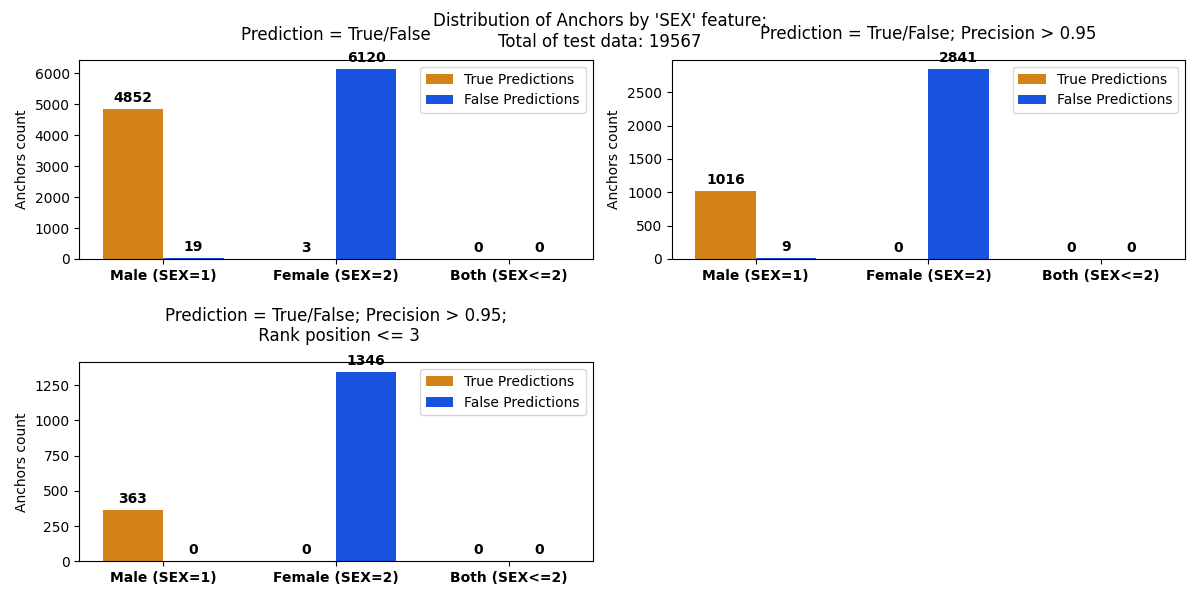
\includegraphics[width=\textwidth]{Images/distribution_folktables/pca_xg_ca_shap.png}
        \caption{Model: XGBoost, XAI method: SHAP}
        \label{fig:distr_xg_ca_shap}
    \end{subfigure}
    \hfill
    \begin{subfigure}[b]{0.9\textwidth}
        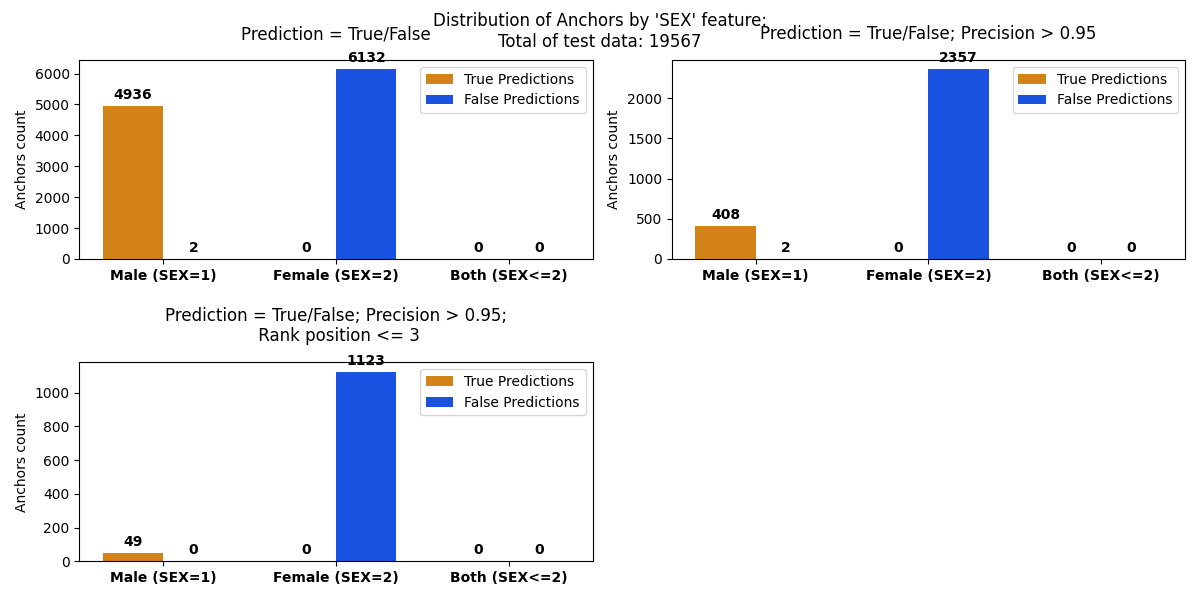
\includegraphics[width=\textwidth]{Images/distribution_folktables/pca_skrub_ca_shap.png}
        \caption{Model: HistGradientBoosting, XAI method: SHAP}
        \label{fig:distr_skrub_ca_shap}
    \end{subfigure}
    \caption{Comparison of the gendered explanations between True and False predictions in the California state (Part 2)}
    \label{fig:distr_ca}
\end{figure}

\begin{figure}[h]
    \centering
    \begin{subfigure}[b]{0.9\textwidth}
        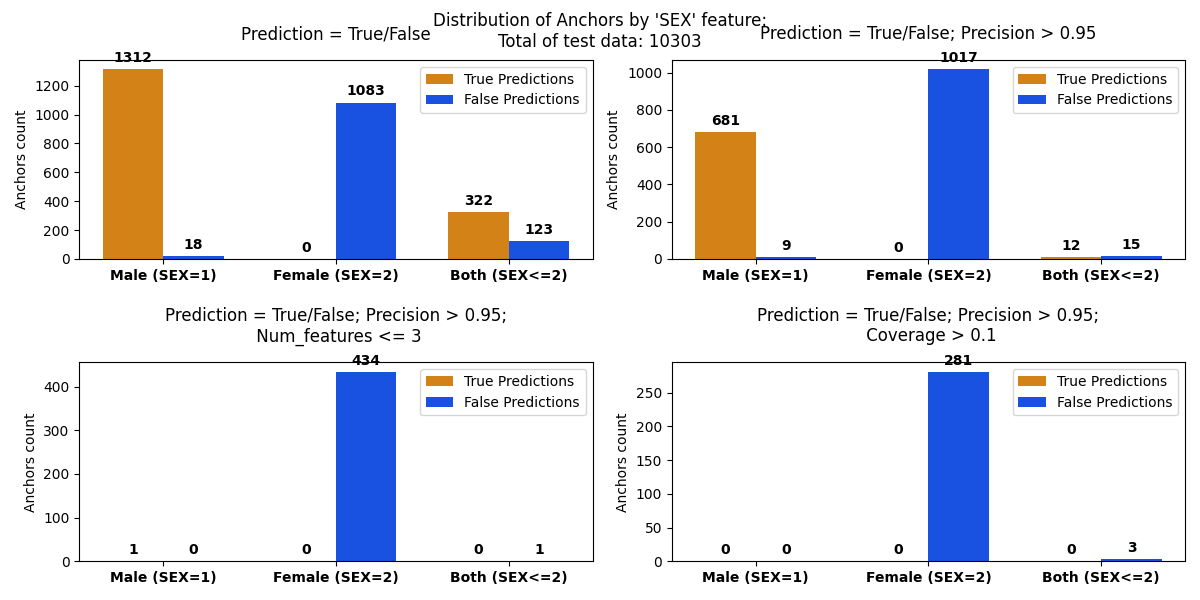
\includegraphics[width=\textwidth]{Images/distribution_folktables/pca_xg_ny_anchors.png}
        \caption{Model: XGBoost, XAI method: Anchors}
        \label{fig:distr_xg_ny_anchors}
    \end{subfigure}
    \hfill
    \begin{subfigure}[b]{0.9\textwidth}
        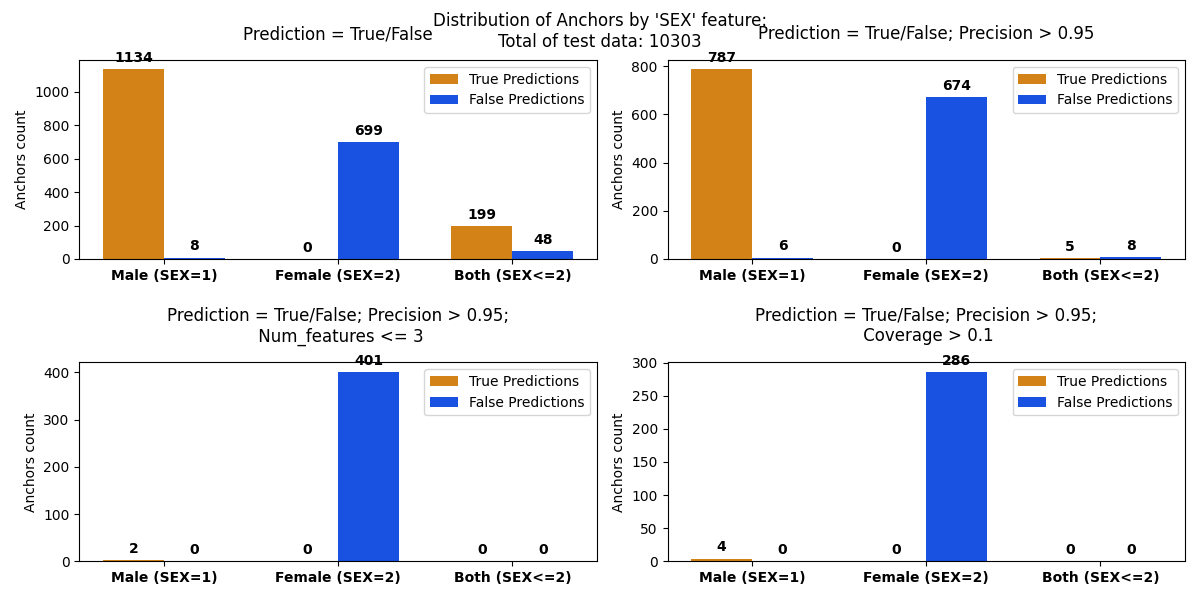
\includegraphics[width=\textwidth]{Images/distribution_folktables/pca_skrub_ny_anchors.png}
        \caption{Model: HistGradientBoosting, XAI method: Anchors}
        \label{fig:distr_skrub_ny_anchors}
    \end{subfigure}
    \caption{Comparison of the gendered explanations between True and False predictions in the New York state (Part 1)}
 \end{figure}

\begin{figure}[h]
    \ContinuedFloat
    \begin{subfigure}[b]{0.9\textwidth}
        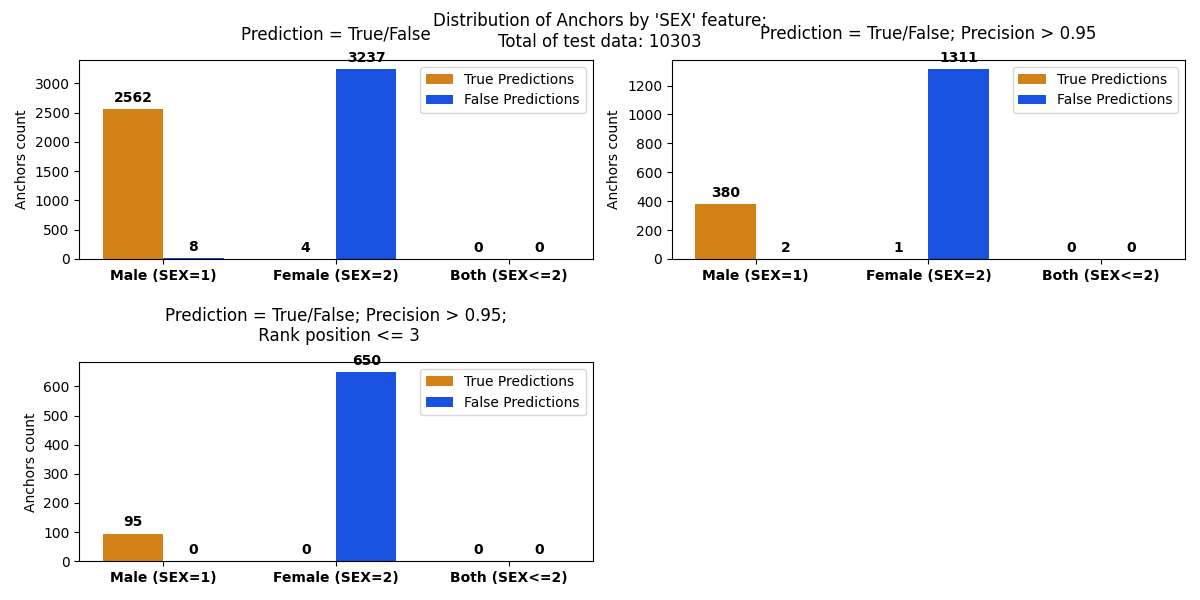
\includegraphics[width=\textwidth]{Images/distribution_folktables/pca_xg_ny_shap.png}
        \caption{Model: XGBoost, XAI method: SHAP}
        \label{fig:distr_xg_ny_shap}
    \end{subfigure}
    \hfill
    \begin{subfigure}[b]{0.9\textwidth}
        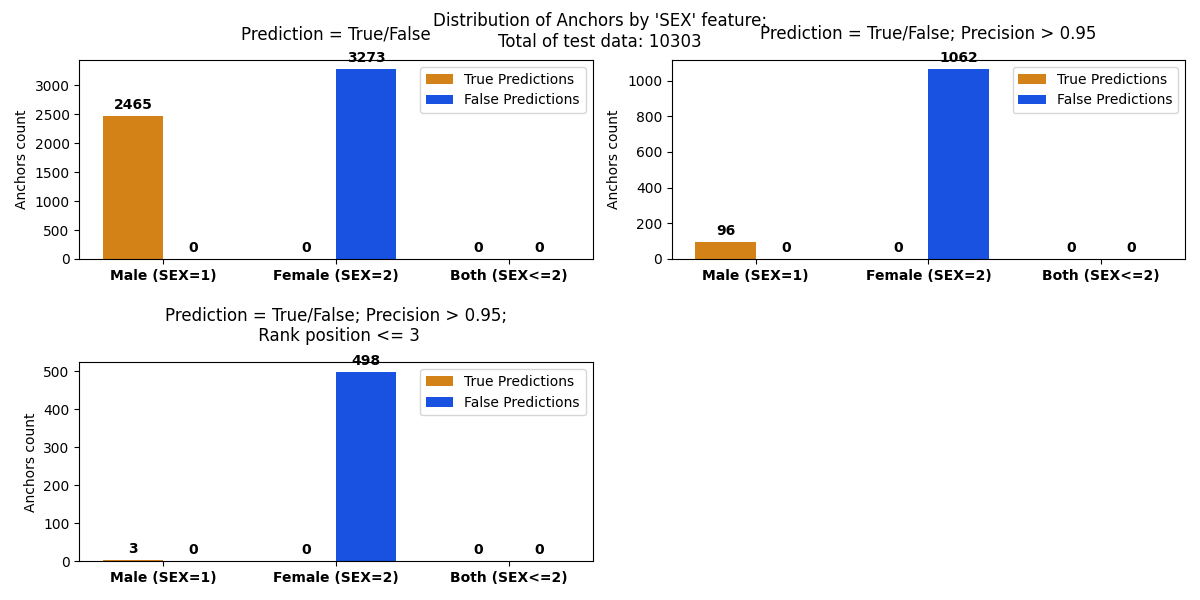
\includegraphics[width=\textwidth]{Images/distribution_folktables/pca_skrub_ny_shap.png}
        \caption{Model: HistGradientBoosting, XAI method: SHAP}
        \label{fig:distr_skrub_ny_shap}
    \end{subfigure}
    \caption{Comparison of the gendered explanations between True and False predictions in the New York state (Part 2)}
    \label{fig:distr_ny}
\end{figure}

Figures \ref{fig:distr_xg_tx_anchors} and \ref{fig:distr_skrub_tx_anchors} show the distribution of the 'SEX' variable in the Anchors generated for the test data of each state for the HistGradientBoosting and XGBoost models, respectively. In other words, the count of gendered anchors, broken down by the value of the 'SEX' variable (Male, Female, or instances where both values are included in the rule) and the model's prediction (True or False).
We also applied filters to understand better the impact of the anchor.

The plots are organized as follows:
\begin{enumerate}
	\item Distribution of True and False predictions among the gendered anchors.
	\item Distribution of True and False predictions (among the gendered anchors) with a precision higher than 95\%.
	\item Distribution of True and False predictions (among the gendered anchors) with a precision higher than 95\% and a rule size limited to three features, meaning a compact anchor.
	\item Distribution of True and False predictions (among the gendered anchors) with a precision higher than 95\% and coverage of the anchors higher than 10\% of the dataset.
\end{enumerate}

We tried to simulate the same tests with SHAP in Figures \ref{fig:distr_xg_tx_shap} and \ref{fig:distr_skrub_tx_shap}, showing the distribution of the 'SEX' variable among instances with positive SHAP values. We applied almost the same filters, apart from the coverage filter because SHAP values do not have a coverage attribute.
The plots are organized as follows:
\begin{enumerate}
	\item Distribution of True and False predictions among the instances with gendered (positive) SHAP values.
	\item Distribution of True and False predictions (among the instances with gendered SHAP values) with a precision higher than 95\%.
	\item Distribution of True and False predictions (among the instances with gendered SHAP values) with a precision higher than 95\% and in which the 'SEX' variable is in the top 3 of the SHAP value ranking.
\end{enumerate}

We can see the results for California and New York data in the Appendix, Figures \ref{fig:distr_ca} and \ref{fig:distr_ny}.

It was interesting to see how many explanations contained gendered anchors or SHAP values, meaning that the technique identified that feature as decisive for the prediction. This implies that if the value of 'SEX' changes, the prediction changes too.

We can also notice that the gendered explanations are divided mainly between women with a false model prediction and men with a true prediction. This reaffirms what the DI metric was showing: this imbalance in the proportion of True predictions for the protected group versus the privileged group.

Analyzing these plots, we discussed that it would be a good idea to analyse the profile of the test dataset to see how the Anchors and SHAP explanations are organized across different groups of people, and also to see which of these two strategies would be more interesting for our case study.

\FloatBarrier

%%%%%%%%%%%%%%%%%%%%%%%%%%%%%%%%%%%%%%%%%%%%%%%%%%%%%%%%%%%%%%%%%%%%%%%%%%%%%%%%%%%%%%%%%%%%%%%%%%%%%%%%%%%%%%%%%%%%%%%
%%%%%%%%%%%%%%%%%%%%%%%%%%%%%%%%%%%%%%%%%%%%%%%%   MÉTÉO   %%%%%%%%%%%%%%%%%%%%%%%%%%%%%%%%%%%%%%%%%%%%%%%%%%%%%%%%%%%%
%%%%%%%%%%%%%%%%%%%%%%%%%%%%%%%%%%%%%%%%%%%%%%%%%%%%%%%%%%%%%%%%%%%%%%%%%%%%%%%%%%%%%%%%%%%%%%%%%%%%%%%%%%%%%%%%%%%%%%%
\subsection{Multi-dimensional Data}
This part of the work was developed in collaboration with Laurent Risser and Météo France. Using the Titan dataset \cite{titandataset} provided by our partners, we explored the structure and composition of meteorological data. For this study, we focused on the Titan data collection for the year 2023.

Our first goal was to understand how meteorological data is organized and combined to produce forecasts. The initial phase involved studying the AROME and ARPÈGE data models and then training a model with a UNetR++-based neural network.

Establishing this solid foundation and successfully training the model was crucial for the next step: applying eXplainable AI (XAI) techniques to the predictions. The aim was to pinpoint the most important channels or specific areas in the input images that drive the model's predictions.

\subsubsection{The Titan Dataset}
This dataset is organized into hourly folders, each containing \textit{.npy} files for all 37 channels from the AROME \cite{arome} and ARPÈGE \cite{arpege} models (see Table \ref{tab:meteo_channels}). In essence, this structure provides a complete set of channel images for every hour (00h to 23h) of every day throughout the entire year of 2023.

Each of these channels represents a specific component of meteorological data, which can be categorized into AROME and ARPÈGE channels representing temperature, humidity, wind, and geopotential at different pressure levels.

\begin{table}[h]
\centering
\caption{Meteorological Data Channels and Their Properties}
\label{tab:meteo_channels}
\begin{tabular}{llll}
\hline
\textbf{Channel Number} & {Channel Name} & \textbf{Description} & \textbf{Altitude/Pressure Level} \\
\hline
1 & aro\_r2\_2m        & Arome relative humidity & 2 metre \\
2 & aro\_t2m\_2m       & Arome temperature & 2 metre \\
3 & aro\_t\_250hpa     & Arome temperature & 250 hPa \\
4 & aro\_t\_500hpa     & Arome temperature & 500 hPa \\
5 & aro\_t\_700hpa     & Arome temperature & 700 hPa \\
6 & aro\_t\_850hpa     & Arome temperature & 850 hPa \\
7 & aro\_tp\_0m        & Arome total precipitation & Surface \\
8 & aro\_u10\_10m      & Arome U wind component & 10 metre \\
9 & aro\_u\_250hpa     & Arome U wind component & 250 hPa \\
10 & aro\_u\_500hpa     & Arome U wind component & 500 hPa \\
11 & aro\_u\_700hpa     & Arome U wind component & 700 hPa \\
12 & aro\_u\_850hpa     & Arome U wind component & 850 hPa \\
13 & aro\_v10\_10m      & Arome V wind component & 10 metre \\
14 & aro\_v\_250hpa     & Arome V wind component & 250 hPa \\
15 & aro\_v\_500hpa     & Arome V wind component & 500 hPa \\
16 & aro\_v\_700hpa     & Arome V wind component & 700 hPa \\
17 & aro\_v\_850hpa     & Arome V wind component & 850 hPa \\
18 & aro\_z\_250hpa     & Arome geopotential & 250 hPa \\
19 & aro\_z\_500hpa     & Arome geopotential & 500 hPa \\
20 & aro\_z\_700hpa     & Arome geopotential & 700 hPa \\
21 & aro\_z\_850hpa     & Arome geopotential & 850 hPa \\
22 & arp\_t\_250hpa     & Arpege temperature & 250 hPa \\
23 & arp\_t\_500hpa     & Arpege temperature & 500 hPa \\
24 & arp\_t\_700hpa     & Arpege temperature & 700 hPa \\
25 & arp\_t\_850hpa     & Arpege temperature & 850 hPa \\
26 & arp\_u\_250hpa     & Arpege U wind component & 250 hPa \\
27 & arp\_u\_500hpa     & Arpege U wind component & 500 hPa \\
28 & arp\_u\_700hpa     & Arpege U wind component & 700 hPa \\
29 & arp\_u\_850hpa     & Arpege U wind component & 850 hPa \\
30 & arp\_v\_250hpa     & Arpege V wind component & 250 hPa \\
31 & arp\_v\_500hpa     & Arpege V wind component & 500 hPa \\
32 & arp\_v\_700hpa     & Arpege V wind component & 700 hPa \\
33 & arp\_v\_850hpa     & Arpege V wind component & 850 hPa \\
34 & arp\_z\_250hpa     & Arpege geopotential & 250 hPa \\
35 & arp\_z\_500hpa     & Arpege geopotential & 500 hPa \\
36 & arp\_z\_700hpa     & Arpege geopotential & 700 hPa \\
37 & arp\_z\_850hpa     & Arpege geopotential & 850 hPa \\
\hline
\end{tabular}
\end{table}

We conducted initial exploratory analyses in Python notebooks to understand the dataset. This involved loading the \textit{.npy} files representing the various channels, examining their structure, and interpreting the meteorological phenomena each one depicts. Examples of these channels are shown in Figure \ref{fig:titan-examples}.

\begin{figure}[h]
    \centering
    \begin{subfigure}[b]{0.3\textwidth}
        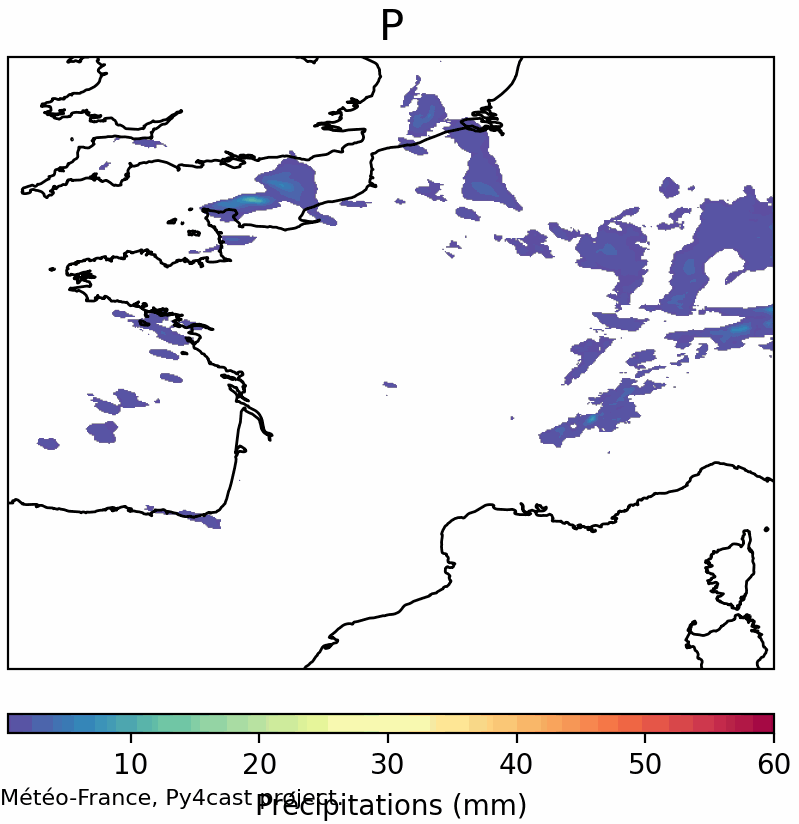
\includegraphics[width=\textwidth]{Images/titan_data_examples/2023111700_feature_aro_tp_0m.png}
        \caption{Feature aro\_tp\_0m}
        \label{fig:titan_aro_tp}
    \end{subfigure}
    \hfill
    \begin{subfigure}[b]{0.3\textwidth}
        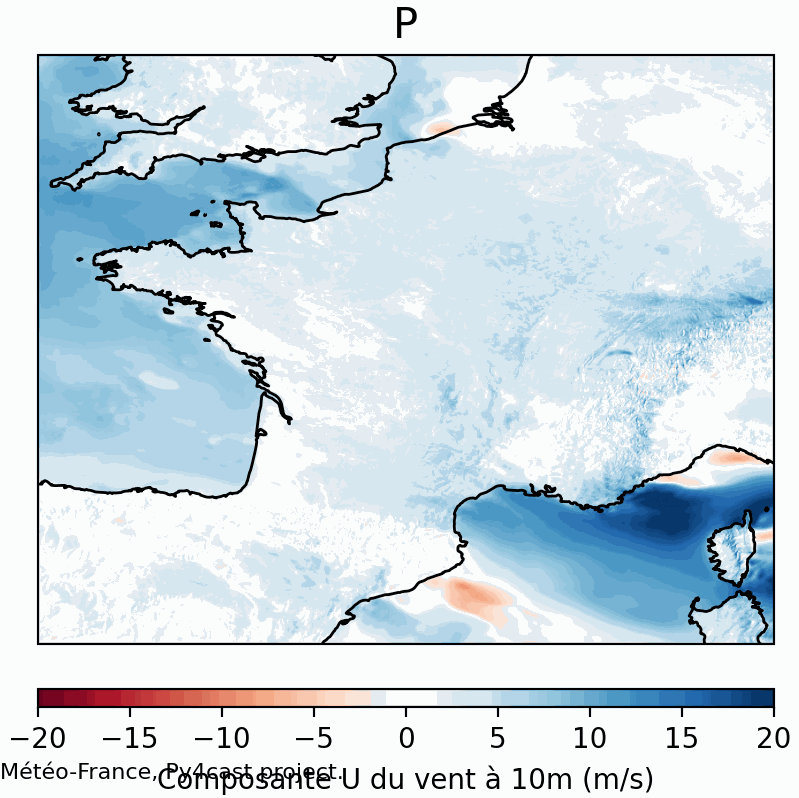
\includegraphics[width=\textwidth]{Images/titan_data_examples/2023111700_feature_aro_u10_10m.png}
        \caption{Feature aro\_u10\_10m}
        \label{fig:titan_aro_u10}
    \end{subfigure}
    \hfill
    \begin{subfigure}[b]{0.3\textwidth}
        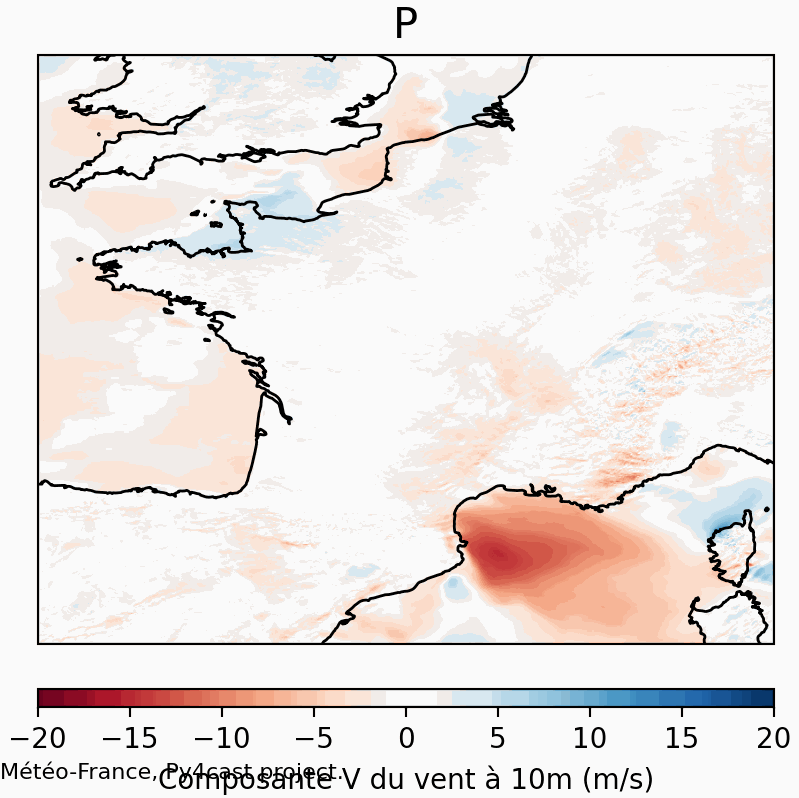
\includegraphics[width=\textwidth]{Images/titan_data_examples/2023111700_feature_aro_v10_10m.png}
        \caption{Feature aro\_v10\_10m}
        \label{fig:titan_aro_v10}
    \end{subfigure}
    \caption{Example of Titan image channels from 17/11/2023}
    \label{fig:titan-examples}
\end{figure}

By analyzing combinations of these components, one can identify and predict impending climatic events. The data can indicate future precipitation (rain or snow), temperature extremes (hot or cold), or the development of severe weather events like storms or flooding in the subsequent hours. For instance, in Figure \ref{fig:titan-examples}, we can identify regions with a high probability of rainfall and observe how wind patterns are likely to advect cloud cover to other areas.

\subsubsection{Training Data}
We first tried to use the \textit{py4cast} Python library \cite{py4cast} to run predictions, but these initial attempts were unsuccessful. As a result, we changed our strategy and began exploring the UNetR++ model using the MFAI Python library \cite{mfai}, developed by Météo France.

The MFAI library provides a framework for training advanced neural network models on meteorological data. We specifically employed it to implement a UNetR++ architecture \cite{unetrpp}. This model was chosen because it combines the strengths of a U-Net, known for its precise spatial segmentation in tasks like medical imaging, with a Vision Transformer (ViT). The ViT backbone is highly effective at capturing long-range dependencies and complex global patterns within the input data—a critical capability for understanding large-scale atmospheric dynamics. The "++" enhancements further refine the architecture for improved performance and efficiency, making it particularly well-suited for processing the high-dimensional, spatial-temporal data characteristic of meteorological fields.

This framework allowed us to investigate viable input and output configurations for weather prediction. It was instrumental in building an understanding of the complexity of meteorological data, the feasibility of training models on it, and the critical choices regarding parameters. The code for these initial experiments is available in the GitHub repository \cite{mfai-experiments}.

This exploratory phase led us to formulate key research questions to guide our work:
\begin{itemize}
\item \textbf{Prediction Target:} What specific meteorological phenomenon should we want to predict?
\item \textbf{Data Selection:} Which input channels are most relevant for this objective, and what should the model output?
\item \textbf{Data Integration:} How should we optimally combine the high-resolution AROME data with the global-scale ARPÈGE data?
\end{itemize}

Fundamentally, the input consists of an ensemble of channels relevant to a specific prediction task, which the model uses to predict the state of those channels at a future time step (e.g., the next hour).

Delving deeper into the integration of AROME and ARPÈGE data, we engaged with the key meteorological concept of training with boundary conditions. This technique is crucial because the AROME model provides high-resolution forecasts over a limited area (a fine mesh), while the ARPÈGE model offers coarser, global-scale (planetary) data. Operational weather forecasting often uses ARPÈGE data to define the boundary conditions for the higher-resolution AROME model. Formally, this can be conceptualized as follows:

Let $t$ be the present time and $t + 1$ be a future time.
\begin{itemize}
	\item Training without boundary conditions:
		\begin{itemize}
			\item Input: $aro_t$ (AROME at time $t$)
			\item Output: $aro_{t+1} - aro_t$ (The change in AROME from $t$ to $t+1$)
		\end{itemize}

	\item Training with boundary conditions:
		\begin{itemize}
			\item Input: $[aro_t, arp_t]$ (AROME and ARPÈGE at time $t$)
			\item Output: $aro_{t+1} - aro_t$ (The change in AROME from $t$ to $t+1$)
		\end{itemize}
\end{itemize}

Integrating the global ARPÈGE data ($arp_t$) as a boundary condition allows the model to incorporate large-scale atmospheric dynamics occurring outside the limited AROME domain, which is essential for generating more accurate predictions within the high-resolution area.

In summary, the data can be combined in two primary ways: a simpler approach using only AROME data, and a more precise, operational-style approach that leverages ARPÈGE data to provide essential boundary conditions.

To address the question of channel selection, we first needed to define a clear prediction objective. We chose precipitation (rain) prediction for its intuitive nature and direct impact. We know intuitively that rainfall is more likely in regions with high cloud cover or where wind patterns are converging and uplifting moisture.

\subsubsection{Using the \textit{py4cast} library}
The \textit{py4cast} library \cite{py4cast} is a Python framework developed by Météo France for short-term weather forecasting. It is specifically designed to work with high-resolution meteorological data from the AROME and ARPÈGE models. The library's core functionality involves processing images from these models to generate predictions for subsequent time steps, typically focused on a one-hour ahead forecast.

We worked in collaboration with Météo France using this library to train a neural network with the UNetR++ model \cite{unetrpp} and the Titan dataset \cite{titandataset} from 2023. This library is very recent, and it was highly valuable for both parties to have an external user test its capabilities. The main objective was to benefit from their library, as it already implemented the weather forecast training pipelines we required, complete with customizable input/output channels and built-in plotting functionalities.

However, as the documentation did not cover many aspects that an external user would not know initially, this process involved significant debugging and led to contributions aimed at improving the library's documentation and overall usability for external users. This challenge was a primary reason our research progress was slower than anticipated.

My role initially involved acting as a beta tester: reading the documentation and attempting to run the UNetR++ trainer. This was necessary because, in practice, Météo France's internal researchers were accustomed to using the library in a pre-configured environment. After several rounds of debugging in collaboration with their team, we successfully managed to run these models and generate the prediction images.


Being able to generate predictions allowed us to proceed with training the models. We trained two distinct models:
\begin{itemize}
	\item \textbf{Complete model}: A model trained with all the available image channels (listed in Table \ref{tab:meteo_channels}) as inputs.
	\item \textbf{Rain model}: A model trained with only the channels most relevant to precipitation (as explained above) as inputs, such as \textit{aro\_tp\_0m}, \textit{aro\_u10\_10m}, and \textit{aro\_v10\_10m}.
\end{itemize} 

\subsubsection{Applying XAI}
In order to apply XAI, we faced significant challenges. A primary obstacle was that standard XAI techniques like Anchors and SHAP are primarily designed for classification models, not regression tasks like weather prediction. Furthermore, applying these perturbation-based methods to multi-channel image data is non-trivial; perturbing individual pixels or channels could generate meteorologically nonsensical input images, rendering the explanations meaningless. We therefore needed to develop a technique that would address these issues.

Focusing on the Anchors framework, we will explore the properties explained in Section \ref{sec:anchors-formalization} to build a new proposition.

We elaborated two extensions of the Anchors formalization, which will be particularly useful for the weather forecasting problem.

\begin{itemize}
	\item Deterministic Precision Constraint: In scenarios where the amount of available data is sufficient to robustly represent the potential distribution $D(z|A)$, or when the estimation of $f(z)$ is computationally expensive, the following simplified optimization problem can be reasonably used:

	\begin{equation}
		\arg \max_{A} {\text{cov}(A) \mid \text{prec}(A) \geq \tau }
		\label{eq:extended-max-cov-anchors}
	\end{equation}

	\item Extension to Regression and Probabilistic Output: The original definition of precision (Eq. \ref{eq:prec-anchors}) is specific to classification tasks. For regression, or to assess the stability of prediction probabilities in classification, the precision measure can be extended as follows:
	
	\begin{equation}
		\text{prec}(A) = \mathbb{E}_{D(z|A)} [\mathbf{1}_{|f(x) - f(z)| > \tau}]
		\label{eq:extended-prec-anchors}
	\end{equation}

	where $\tau$ is a threshold above which the conditions of A are supposed to have a significant impact.
\end{itemize}

It is now crucial to define the specific subject of our explanations. Explaining the entire prediction $\widetilde{x_{t+1}}$ appears both technically intractable and, in our view, not particularly useful. Instead, we will focus on answering a more targeted question: why is $\widetilde{x_{t+1}}(i, j, c) \in R$? Here, $R$ represents a specific range of values. For instance, $(i, j)$ could denote the geographical coordinates of a city and $c$ the output channel representing the predicted rainfall in millimeters at that location for the next hour.

In this framework, defining $R = [ 1, +\infty [$ would allow us to explain why at least light rain is predicted locally. Alternatively, setting $R = [10, +\infty [$ would help explain the prediction of heavy rainfall.

To align with the classification framework established in Section \ref{sec:anchors-formalization}, we define a function $g_{i,j,c,R}(.)$ that transforms the regression output into a binary classification problem:
\begin{equation}
	g_{i,j,c,R}(\widetilde{x_{t+1}}) = \mathbf{1}_{\widetilde{x_{t+1}}(i, j, c) \in R}
\end{equation}

In summary, using Eq. \ref{eq:extended-max-cov-anchors}, we will explain the decisions $g_{i,j,c,R}(f(x_t))$ by evaluating the model on perturbed inputs $z$ similar to $x_t$. This approach raises two key questions:
\begin{itemize}
	\item Which channels of $z$ will be perturbed to generate the counterfactuals?
	\item Which types of conditions of $A$ can be considered on weather forecasting data, to formally measure the precisions and coverages of potentials anchors A?
\end{itemize}

Our two main difficulties in addressing the key questions above are:
\begin{itemize}
\item The dimensionality of the input $x_t$ is very large (with $p$ typically on the order of $500 \times 500 \times 20$).
\item Each model inference $f(z)$ or $f(x_t)$ requires a non-negligible amount of computational time.
\end{itemize}

Therefore, to generate pertinent explanations with reasonable computational resources, it is mandatory to sample perturbations $z$ using strong priors that guide the exploration towards meaningful differences from $x_t$.

What strategies can we use?
\begin{enumerate}
\item Leverage Spatial Structure: Unlike tabular data, we can exploit the spatial relationships between variables when defining predicates in $A$.
\item Define Clear Counterfactuals: The instances $z$ should be counterfactual versions of $x_t$, where the differences are explicitly defined by quantifiable relationships (e.g., concerning spatial locations, channel values, or local perturbations). The conditions in anchor $A$ must be able to formally express these relationships.
\item Focus on Local Neighborhood: Since the explanation targets a specific spatial location $(i, j)$, it is reasonable to sample $z$ by introducing differences within the neighborhood of $(i, j)$.
\item Utilize Domain Knowledge for Sampling: For each channel $c$—and potentially for each location $(i, j)$, hour, or season—domain knowledge can provide plausible value ranges for sampling $z$. Working with centered and reduced data (as is the case in py4cast) may simplify this generation process, as the range of potential values is broadly controlled and normalized.
\item Decouple Computation via a Table: The differences between each sampled $z$ and $x_t$ should be cataloged in a table. This approach would allow an external script to compute the Precision and Coverage measures for potential anchors $A$ using pre-computed model outputs. If executed properly, this method would require no modifications to the core py4cast code.
\end{enumerate}

\subsubsection{Proposed Solution}
We suppose that $g_{i,j,c,R}(f(x_t)) == 1$ and we want to explain why using anchors. We will sample $K$ different counterfactual observations ${z_k}$, for $k \in {1, \ldots , K}$, by generating perturbations based on the following quantified conditions:

\begin{itemize}
	\item \textbf{Center of Perturbation $(\widehat{i_k}, \widehat{j_k})$:} The epicenter of the perturbation should be close to the target location $(i, j)$ and lie within the spatial domain of the image. We can sample this center from a distribution, for instance $\widehat{i_k} \sim \mathcal{N}(i, \sigma_d)$ and $\widehat{j_k} \sim \mathcal{N}(j, \sigma_d)$, where $\sigma_d$ is a hyperparameter controlling the typical spatial scale of the perturbations. If the sampled coordinate falls outside the valid domain, it is projected to the nearest pixel on the grid.
	
	\item \textbf{Channel of Perturbation $\widehat{c_k}$:} The channel to be perturbed can be sampled uniformly from the available channels.
	
	\item \textbf{Perturbation Value $\widehat{v_k}$:} This defines the new value for the pixel at the chosen location and channel, i.e., $z_k(\widehat{i_k}, \widehat{j_k}, \widehat{c_k}) = \widehat{v_k}$. Assuming the channels of $x_t$ are centered and reduced, we can sample the new value from a distribution such as $\widehat{v_k} \sim \mathcal{N}(\mu, \sigma_v)$, where $\mu$ and $\sigma_v$ are hyperparameters. The maximum and minimum possible values for $\widehat{v_k}$ must be bounded by the physical limits (min/max) of the channel $\widehat{c_k}$ to ensure the generated counterfactual $z_k$ remains meteorologically plausible.
\end{itemize}

It can be remarked that altering the value of a single pixel in $x_t$ may have a negligible impact on the prediction $g_{i,j,c,R}(f(x_t))$ and often lacks physical realism. To address this, we introduce a second hyperparameter, $\sigma_e$, which models the spatial extent of the perturbation. The procedure for generating a counterfactual instance $z_k$ is then as follows:
\begin{itemize}
	\item \textbf{Unaffected Channels:} For all channels $c \neq \widehat{c_k}$, the data remains unchanged: $z_k(:, :, c) = x_t(:, :, c)$.
	
	\item \textbf{Mask Creation:} A mask $m \in \mathbb{R}^{I \times J}$ is generated. Its values are initially drawn from a 2D Gaussian distribution centered at $(\widehat{i_k}, \widehat{j_k})$ with covariance matrix $\begin{bmatrix} \sigma_e & 0 \ 0 & \sigma_e \end{bmatrix}$. These values are then linearly rescaled to the interval $[0, 1]$.
	
	\item \textbf{Application:} The perturbed channel $\widehat{c_k}$ in $z_k$ is created by a mask-based blending between the original values and the new value $\widehat{v_k}$:
	\begin{equation}
		z_k(\overline{i} , \overline{j} , \widehat{c_k}) = m(\overline{i} , \overline{j} ) * \widehat{v_k} + (1 - m(\overline{i} , \overline{j})) * x_t(\overline{i} , \overline{j}, \widehat{c_k})
		\label{eq:anchor-perturbation}
	\end{equation}
	for all $\overline{i} \in {1, \ldots, I}$ and $\overline{j} \in {1, \ldots, J}$.
\end{itemize}

Once all counterfactual observations ${z_k}$ are generated, we compute the corresponding model outputs $g_{i,j,c,R}(f(z_k))$. The anchor explanation process can then be performed by treating the set of perturbation parameters ($\widehat{i_k}, \widehat{j_k}, \widehat{c_k}, \widehat{v_k}$) and their outcomes $g_{i,j,c,R}(f(z_k))$ as tabular data for analysis.

% Falar sobre gradients e como nao conseguimos extrai-los por causa do Lightning
\section{Results}
\subsection{Fairness Analysis on Tabular Data}
In the context of the work done on the Folktables, we decided to explore the profiles for which the XAI explanations were showing gendered anchors or gendered SHAP values. To move beyond a purely tabular analysis and gain a holistic, spatial understanding of these profiles, we employed a classic dimensionality reduction technique.

For this purpose, we applied Principal Component Analysis (PCA) \cite{pca-mackiewicz} with 2 components to the test dataset. This technique projects the high-dimensional feature space onto a two-dimensional plane defined by the principal components that capture the maximum variance within the data. This projection is crucial as it allows us to:

\begin{itemize}
    \item Assess Data Consistency: Compare the distributions of the training and test sets to ensure the stability and representativeness of our analysis, guarding against artifacts caused by data drift.

    \item Visualize Complex Relationships: See how individuals are spatially distributed based on their combined socioeconomic and demographic characteristics (e.g., age, education, occupation, marital status, ...).
    
    \item Identify Macro-Groups: Observe if individuals with similar XAI explanation patterns (e.g., gendered anchors) naturally coalesce into distinct groups within this reduced space, suggesting underlying demographic substructures that the model is drawing.
\end{itemize}


Figure \ref{fig:pca_tx} show the PCA of the Texas state made for four configurations. Model trained with XGBoost or HistGradientBoosting and explained with the Anchors or SHAP method.
On the left we have the test data in contrast to the training data, confirming no significant discrepancy, and on the right the PCA of the test data in contrast with the gendered explanation found within it. The PCA applied on test data of California and New York can be found in Figures \ref{fig:pca_ca} and \ref{fig:pca_ny}. Applying the PCA is a first step to see where the gendered explanations are concentrated and how each XAI method draw it.

\begin{figure}[h]
    \centering
    \begin{subfigure}[b]{0.9\textwidth}
        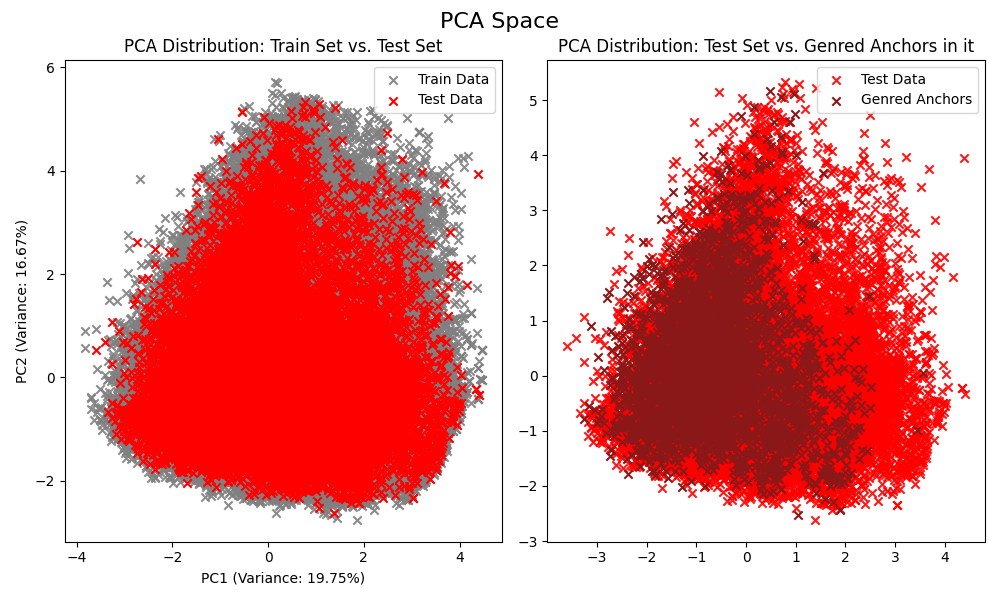
\includegraphics[width=\textwidth]{Images/pca/pca_xg_ca_anchors.png}
        \caption{Model: XGBoost, XAI method: Anchors}
        \label{fig:pca_xg_ca_anchors}
    \end{subfigure}
    \hfill
    \begin{subfigure}[b]{0.9\textwidth}
        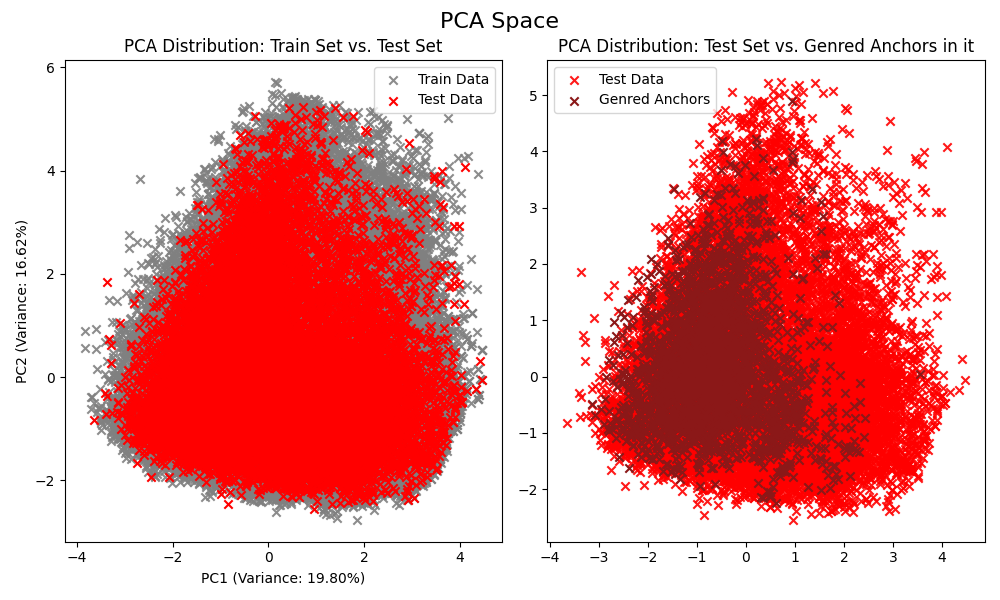
\includegraphics[width=\textwidth]{Images/pca/pca_skrub_ca_anchors.png}
        \caption{Model: HistGradientBoosting, XAI method: Anchors}
        \label{fig:pca_skrub_ca_anchors}
    \end{subfigure}
    \caption{PCA of the test dataset in the California state (Part 1)}
 \end{figure}

\begin{figure}[h]
    \ContinuedFloat
    \begin{subfigure}[b]{0.9\textwidth}
        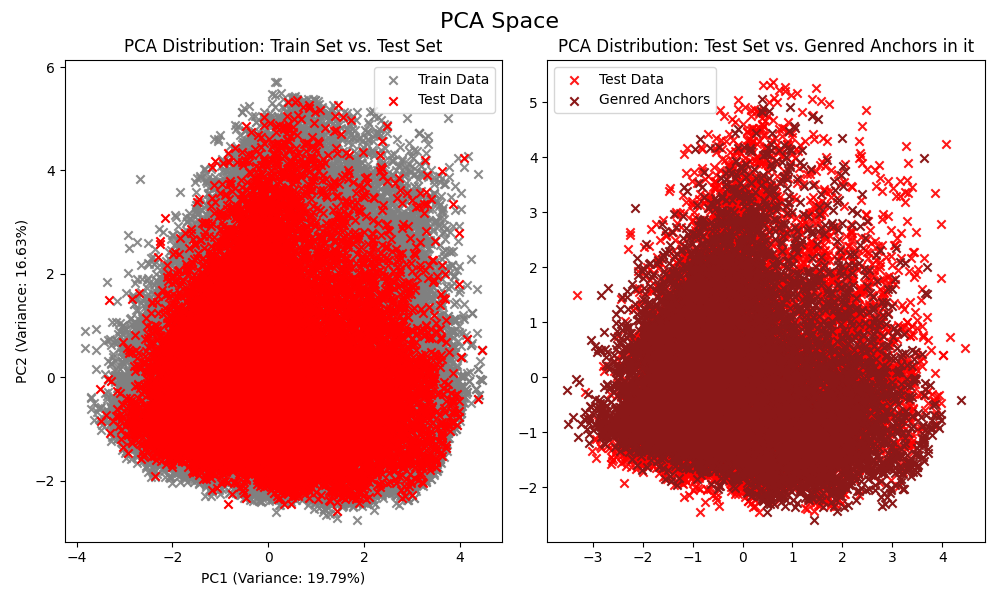
\includegraphics[width=\textwidth]{Images/pca/pca_xg_ca_shap.png}
        \caption{Model: XGBoost, XAI method: SHAP}
        \label{fig:pca_xg_ca_shap}
    \end{subfigure}
    \hfill
    \begin{subfigure}[b]{0.9\textwidth}
        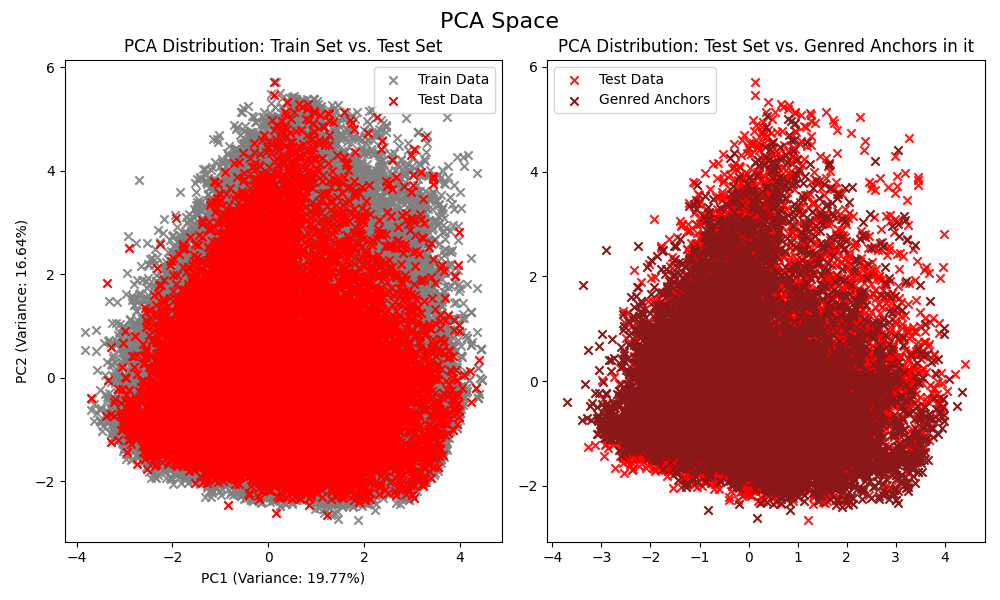
\includegraphics[width=\textwidth]{Images/pca/pca_skrub_ca_shap.png}
        \caption{Model: HistGradientBoosting, XAI method: SHAP}
        \label{fig:pca_skrub_ca_shap}
    \end{subfigure}
    \caption{PCA of the test dataset in the California state (Part 2)}
    \label{fig:pca_ca}
\end{figure}
    


\begin{figure}[h]
    \centering
    \begin{subfigure}[b]{0.9\textwidth}
        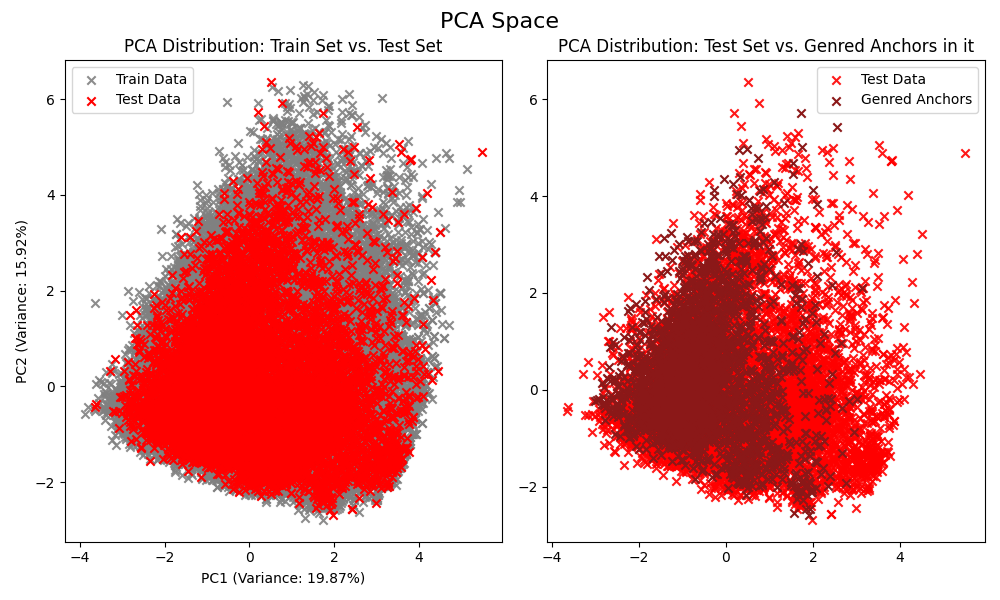
\includegraphics[width=\textwidth]{Images/pca/pca_xg_ny_anchors.png}
        \caption{Model: XGBoost, XAI method: Anchors}
        \label{fig:pca_xg_ny_anchors}
    \end{subfigure}
    \hfill
    \begin{subfigure}[b]{0.9\textwidth}
        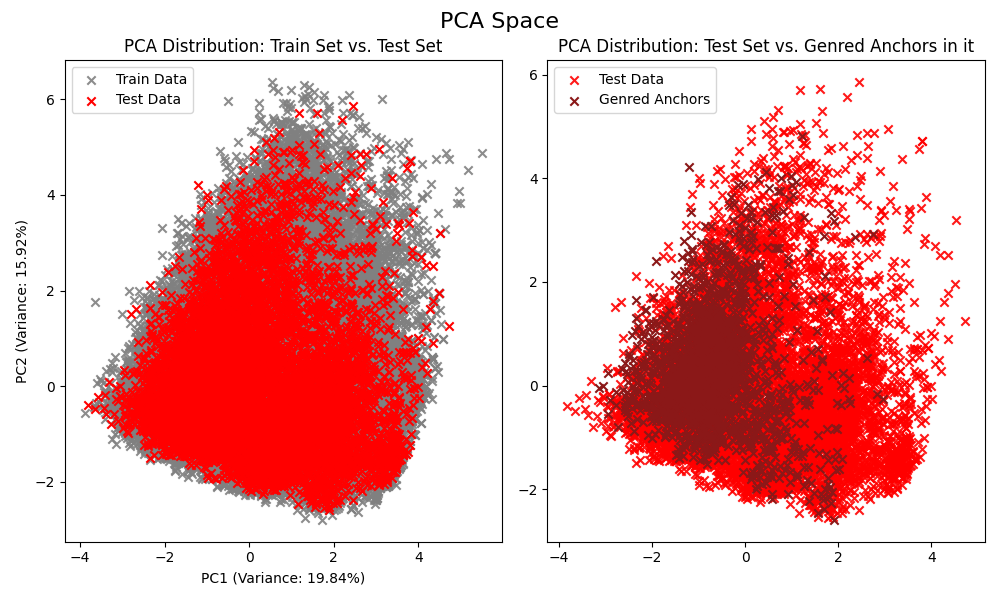
\includegraphics[width=\textwidth]{Images/pca/pca_skrub_ny_anchors.png}
        \caption{Model: HistGradientBoosting, XAI method: Anchors}
        \label{fig:pca_skrub_ny_anchors}
    \end{subfigure}
\caption{PCA of the test dataset in the New York state (Part 1)}
 \end{figure}

\begin{figure}[h]
    \ContinuedFloat
    \begin{subfigure}[b]{0.9\textwidth}
        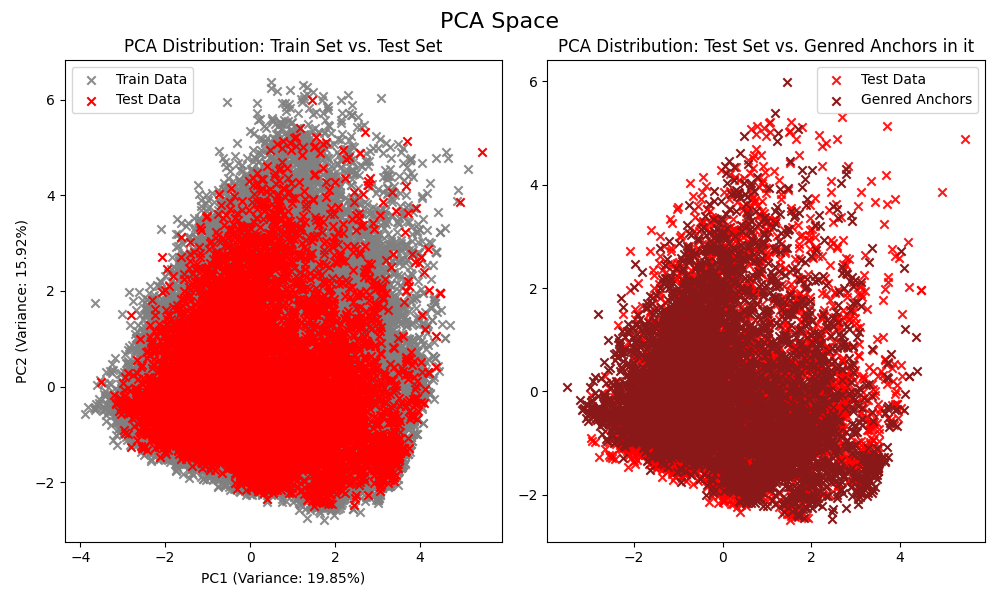
\includegraphics[width=\textwidth]{Images/pca/pca_xg_ny_shap.png}
        \caption{Model: XGBoost, XAI method: SHAP}
        \label{fig:pca_xg_ny_shap}
    \end{subfigure}
    \hfill
    \begin{subfigure}[b]{0.9\textwidth}
        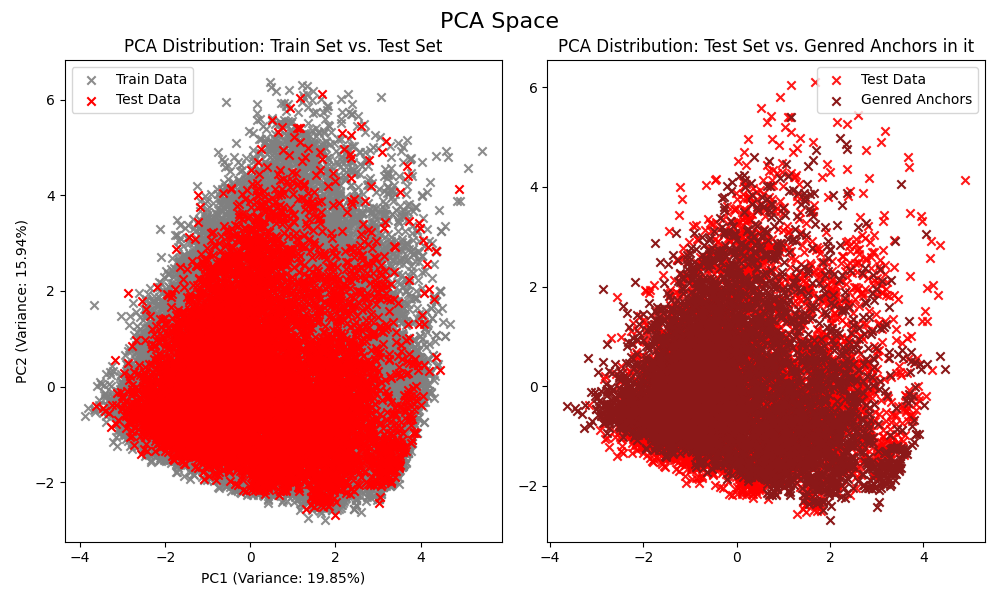
\includegraphics[width=\textwidth]{Images/pca/pca_skrub_ny_shap.png}
        \caption{Model: HistGradientBoosting, XAI method: SHAP}
        \label{fig:pca_skrub_ny_shap}
    \end{subfigure}
    \caption{PCA of the test dataset in the New York state (Part 2)}
    \label{fig:pca_ny}
\end{figure}

The next step is to formally define and label the distinct profiles observed in the PCA projection, we subsequently applied K-means clustering with three clusters \cite{kmeans-pca-ding}. This classic technique complements the PCA by algorithmmatically identifying dense regions of data points, thus quantitatively defining the macro-groups suggested by the visual inspection. This two-step approach—unsupervised projection followed by clustering—provides a robust, data-driven foundation for interpreting the XAI results. It allows us to move from observing vague groupings to analyzing well-defined clusters, each representing a specific demographic and socioeconomic profile prevalent in the data.

In Figure \ref{fig:clusters_tx} we can see the clustered PCA with the same configurations used in the figures described in Section \ref{met:fairness-xai}. The clustered PCA applied to the test data of California and New York can be found in Figures \ref{fig:clusters_ca} and \ref{fig:clusters_ny}.

\begin{figure}[h]
    \centering
    \begin{subfigure}[b]{1.0\textwidth}
        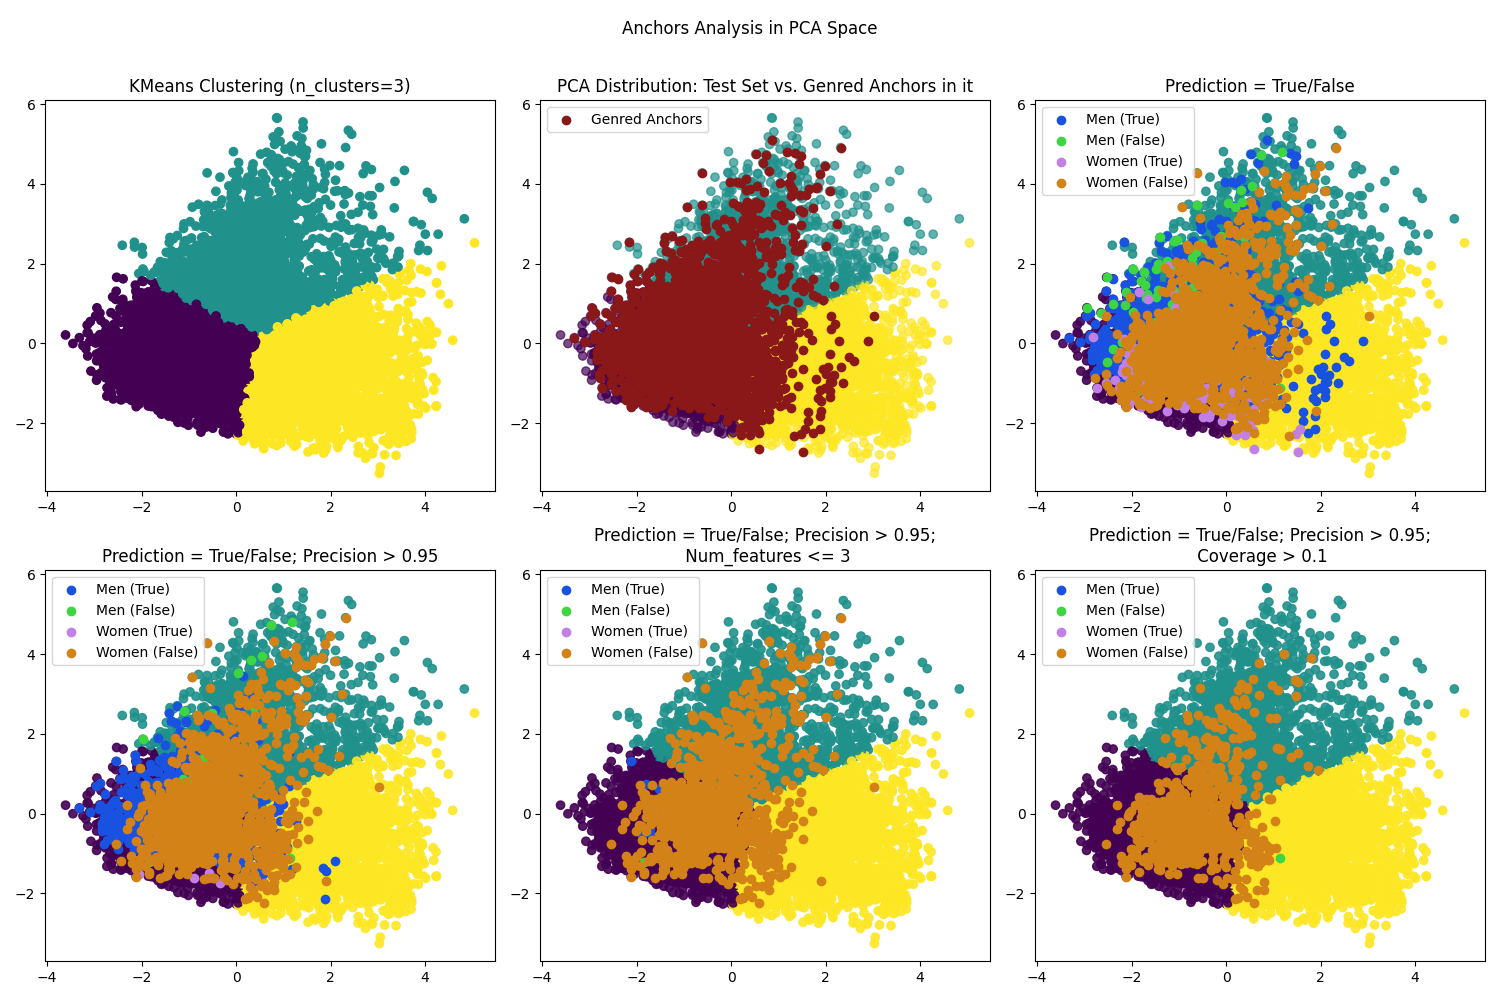
\includegraphics[width=\textwidth]{Images/clustered_pca/clusters_xg_tx_anchors.png}
        \caption{Model: XGBoost, XAI method: Anchors}
        \label{fig:clusters_xg_tx_anchors}
    \end{subfigure}

    \begin{subfigure}[b]{1.0\textwidth}
        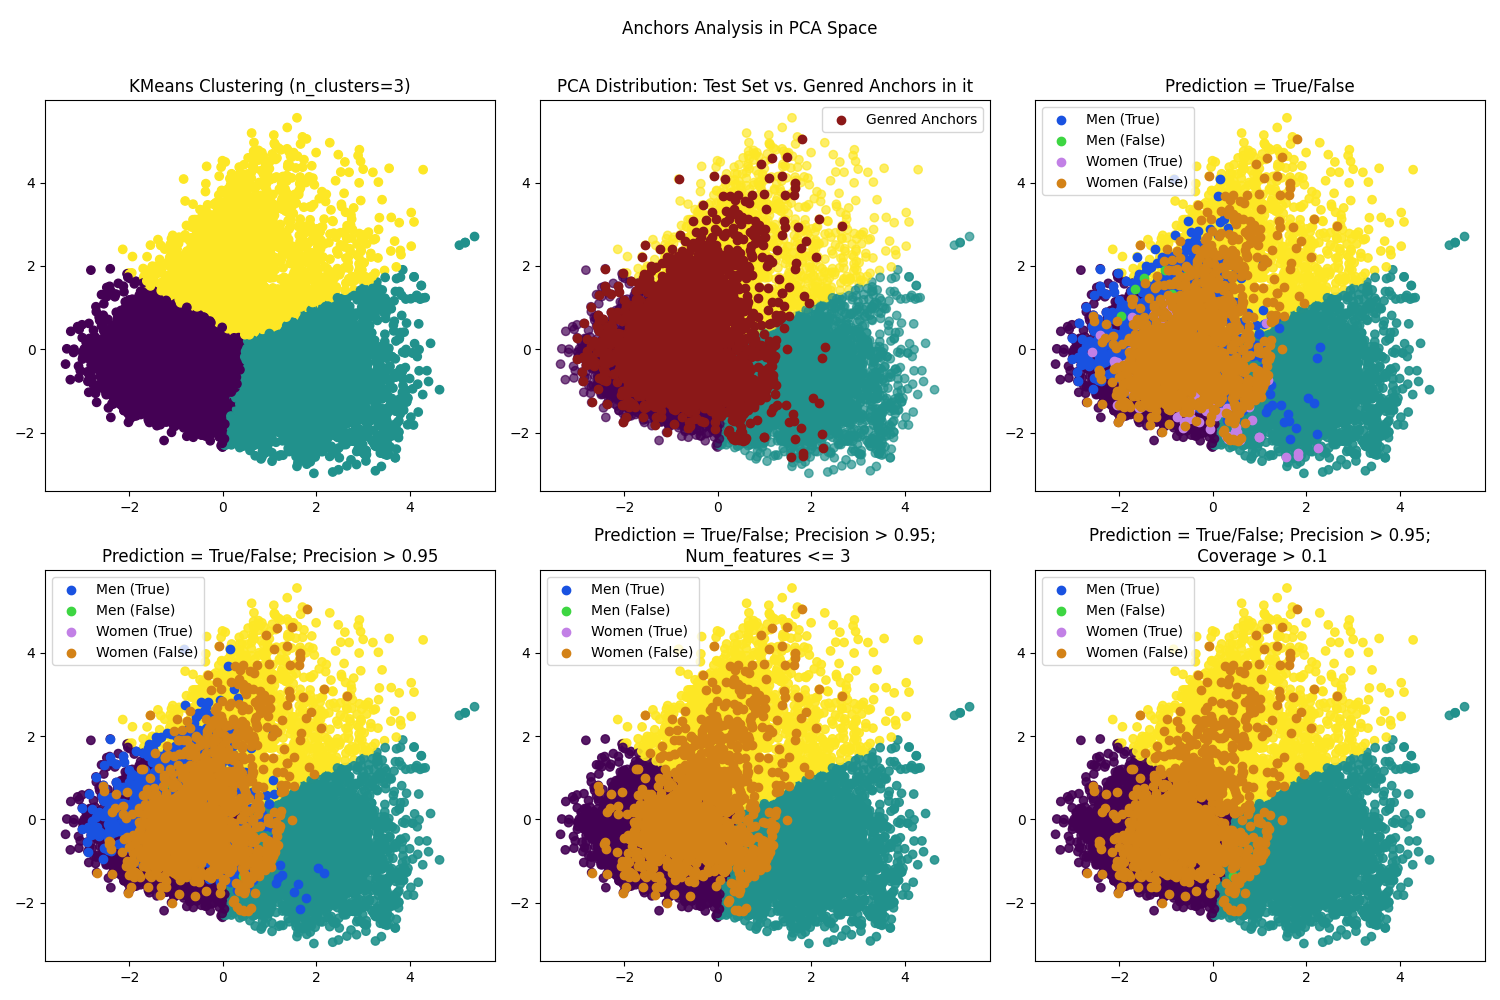
\includegraphics[width=\textwidth]{Images/clustered_pca/clusters_skrub_tx_anchors.png}
        \caption{Model: HistGradientBoosting, XAI method: Anchors}
        \label{fig:clusters_skrub_tx_anchors}
    \end{subfigure}
    \caption{Comparison of the clustered PCA in the Texas state, putting in evidence gendered explanations (Part 1)}
\end{figure}

\begin{figure}[h]
    \ContinuedFloat
    \begin{subfigure}[b]{1.0\textwidth}
        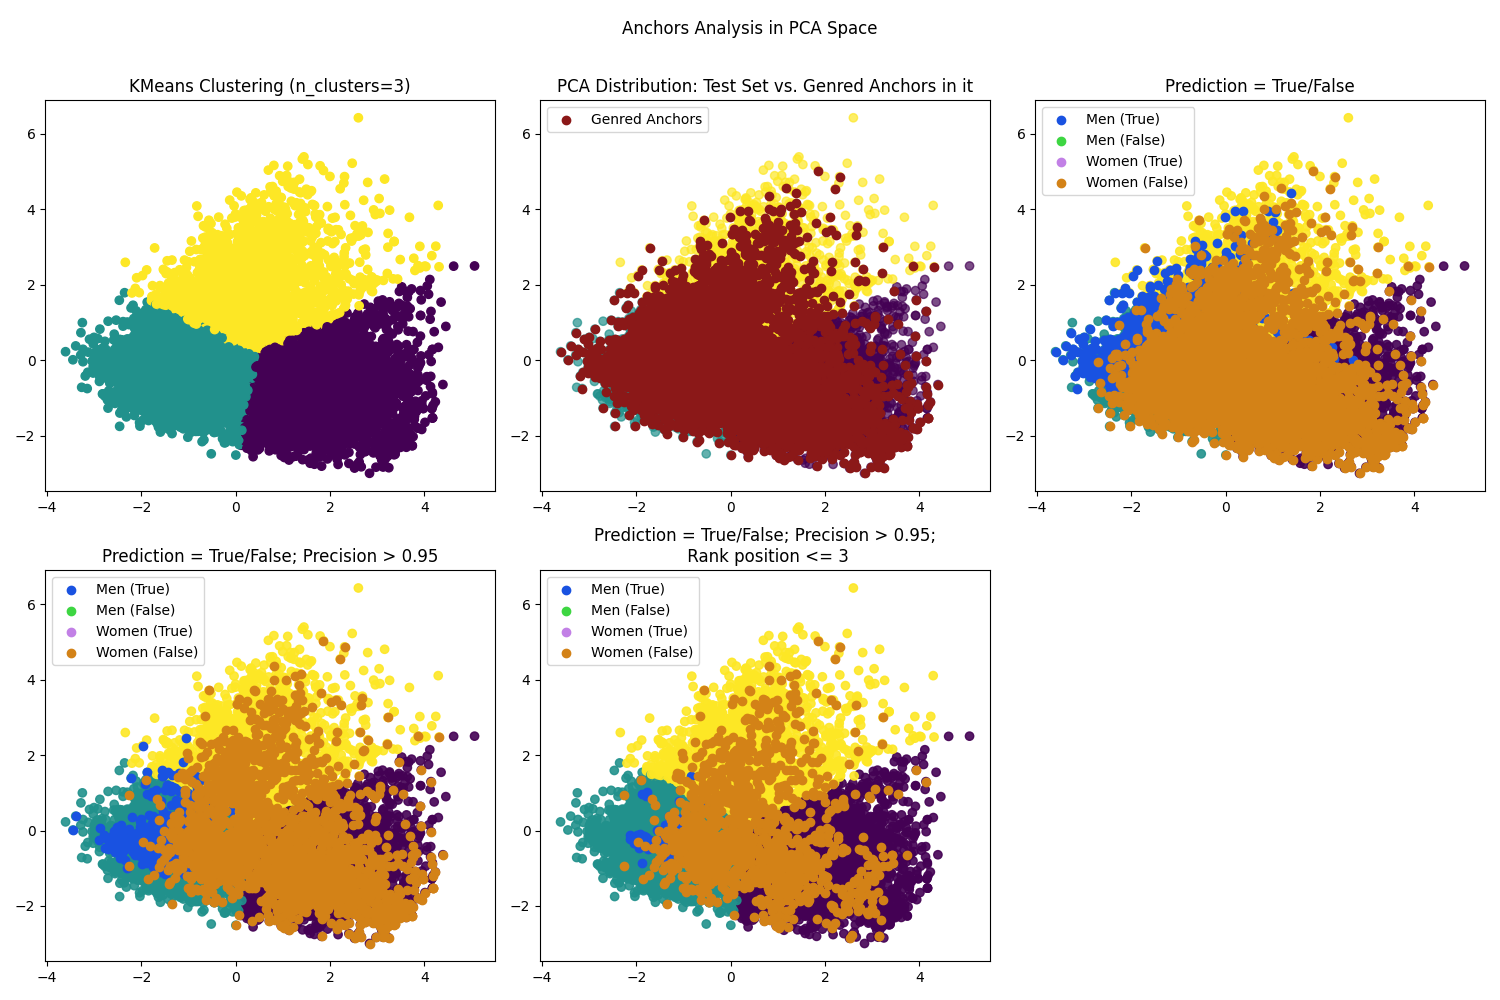
\includegraphics[width=\textwidth]{Images/clustered_pca/clusters_xg_tx_shap.png}
        \caption{Model: XGBoost, XAI method: SHAP}
        \label{fig:clusters_xg_tx_shap}
    \end{subfigure}

    \begin{subfigure}[b]{1.0\textwidth}
        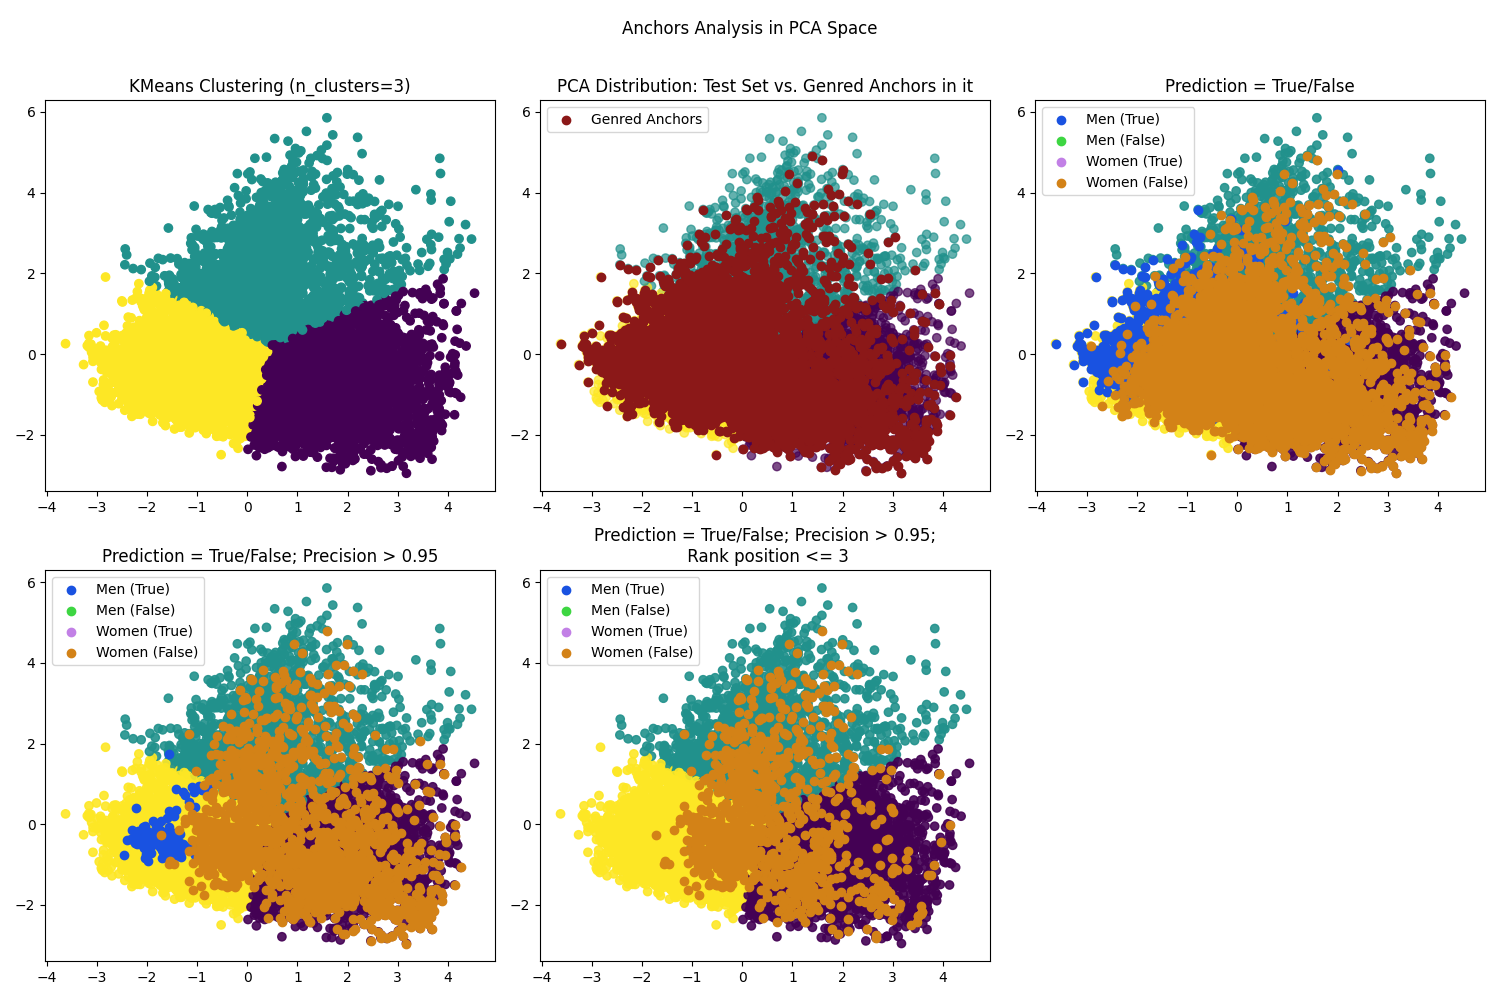
\includegraphics[width=\textwidth]{Images/clustered_pca/clusters_skrub_tx_shap.png}
        \caption{Model: HistGradientBoosting, XAI method: SHAP}
        \label{fig:clusters_skrub_tx_shap}
    \end{subfigure}

    \caption{Comparison of the clustered PCA in the Texas state, putting in evidence gendered explanations (Part 2)}
    \label{fig:clusters_tx}
\end{figure}

Figures \ref{fig:clusters_xg_tx_anchors} and \ref{fig:clusters_skrub_tx_anchors} build for the Anchors XAI method are organized as follows:
\begin{enumerate}
    \item KMeans clustering with 3 clusters of the PCA of test data
    \item Contrast of the gendered anchors with the clustering of the PCA
	\item Contrast of gendered anchors with the clustering organized by category (Men with true predictions, en with False predictions, Women with true predictions and Women with false predictions)
	\item Contrast of gendered anchors with the clustering organized by category, and filtering the anchors with a precision higher than 95\%.
	\item Contrast of gendered anchors with the clustering organized by category, and filtering the anchors with a precision higher than 95\% and a rule size limited to three features (meaning a compact anchor).
	\item Contrast of gendered anchors with the clustering organized by category, and filtering the anchors with a precision higher than 95\% and coverage of the anchors higher than 10\% of the dataset.
\end{enumerate}

Figures \ref{fig:clusters_xg_tx_shap} and \ref{fig:clusters_skrub_tx_shap} build for the SHAP XAI method are organized as follows:
\begin{enumerate}
    \item KMeans clustering with 3 clusters of the PCA of test data
    \item Contrast of the gendered SHAP values with the clustering of the PCA
	\item Contrast of gendered SHAP values with the clustering organized by category (Men with true predictions, en with False predictions, Women with true predictions and Women with false predictions)
	\item Contrast of gendered SHAP values with the clustering organized by category, and filtering the predictions with a precision higher than 95\%.
	\item Contrast of gendered SHAP values with the clustering organized by category, and filtering the predictions with a precision higher than 95\% and the SHAP values in which the 'SEX' variable is in the top 3 of the ranking.
\end{enumerate}

The code for all this analysis and results was developed to be a Python library and can be found in the GitHub repository \cite{fairness-experiments}.

\FloatBarrier

%%%%%%%%%%%%%%%%%%%%%%%%%%%%%%%%%%%%%%%%%%%%%%%%%%%%%%%%%%%%%%%%%%%%%%%%%%%%%%%%%%%%%%%%%%%%%%%%%%%%%%%%%%%%%%%%%%%%%%%
%%%%%%%%%%%%%%%%%%%%%%%%%%%%%%%%%%%%%%%%%%%%%%%%   MÉTÉO   %%%%%%%%%%%%%%%%%%%%%%%%%%%%%%%%%%%%%%%%%%%%%%%%%%%%%%%%%%%%
%%%%%%%%%%%%%%%%%%%%%%%%%%%%%%%%%%%%%%%%%%%%%%%%%%%%%%%%%%%%%%%%%%%%%%%%%%%%%%%%%%%%%%%%%%%%%%%%%%%%%%%%%%%%%%%%%%%%%%%

\subsection{"Anchors Regression" applied on Meteorological Data}
Given the methodology previously exposed, we constructed our solution using the framework of \textit{py4cast}.
Based on the objective of rain prediction, we prioritized a subset of channels to simplify the initial problem complexity. We built a more controlled environment with only three channels, the ones most directly associated with the physics of rainfall in the lower atmosphere, such as:
\begin{itemize}
	\item \textit{aro\_tp\_0m} (Total Precipitation)
	\item \textit{aro\_u10\_10m} (Zonal wind component at 10m)
    \item \textit{aro\_v10\_10m} (Meridional wind component at 10m)
\end{itemize}

In that way, we could test the approach with simpler data and adapt the hyperparameters before progressing to models using twenty channels.

Figure \ref{fig:titan-rain-perturbations} shows examples of how we perturb the channels with the masks for each one of the three channels to generate the counterfactuals.

\begin{figure}[h]
    \centering
    \begin{subfigure}[b]{0.32\textwidth}
        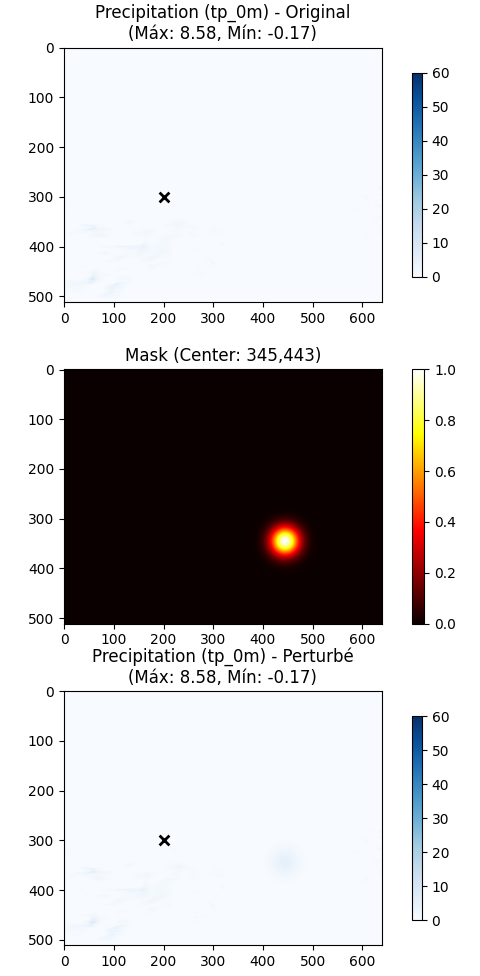
\includegraphics[width=\textwidth]{Images/titan_rain_perturbations/perturbed_c_tp_0m.png}
        \caption{Channel aro\_tp\_0m}
        \label{fig:titan_perturbed_aro_tp}
    \end{subfigure}
    \hfill
    \begin{subfigure}[b]{0.32\textwidth}
        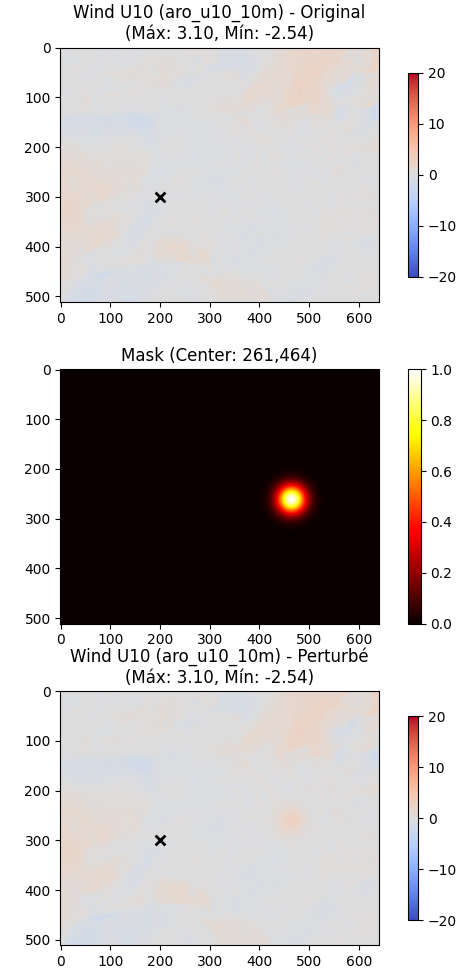
\includegraphics[width=\textwidth]{Images/titan_rain_perturbations/perturbed_c_u10_10m.png}
        \caption{Channel aro\_u10\_10m}
        \label{fig:titan_perturbed_aro_u10}
    \end{subfigure}
    \hfill
    \begin{subfigure}[b]{0.32\textwidth}
        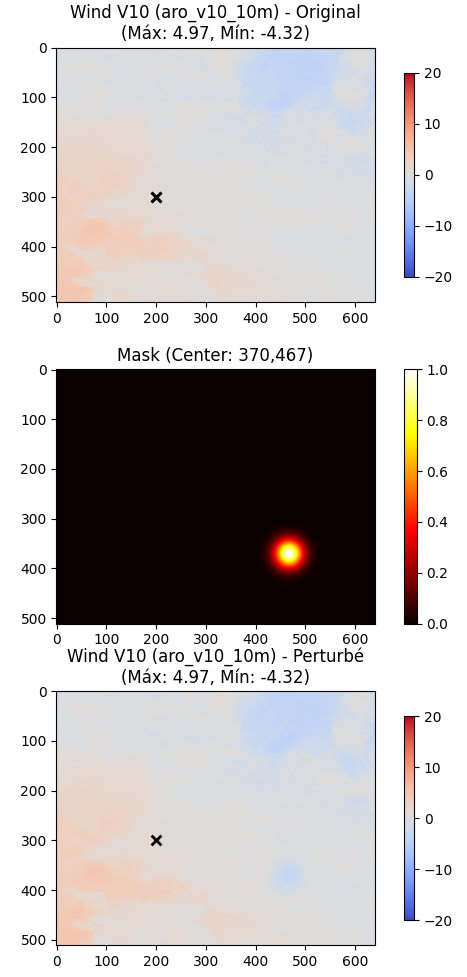
\includegraphics[width=\textwidth]{Images/titan_rain_perturbations/perturbed_c_v10_10m.png}
        \caption{Channel aro\_v10\_10m}
        \label{fig:titan_perturbed_aro_v10}
    \end{subfigure}
    \caption{Example of counterfactuals of Titan image channels from 18/11/2023}
    \label{fig:titan-rain-perturbations}
\end{figure}

Thus, we implemented a loop to generate $K$ counterfactuals for each prediction, balancing time and computational cost with the need for a sufficient number of counterfactuals to produce solid results.

The following configurations were used for generating the anchors:
\begin{itemize}
    \item Sampling period: November 2023.
    \item Number of counterfactuals: $K = 300$.
    \item Center of target location: Centered on $(i, j)$.
    \begin{itemize}
        \item Spatial extent of the center of the perturbation mask: $\sigma_d = 150$ pixels.
    \end{itemize}
    \item Center of perturbation mask: Centered on $(\widehat{i_k}, \widehat{j_k})$.
    \begin{itemize}
        \item Spatial extent of the perturbation mask: $\sigma_e = 20$ pixels.
    \end{itemize}
    \item Prediction difference threshold: $\epsilon = 0.05$ (i.e., the prediction is considered to have changed if it varies by more than 5\%).
\end{itemize}

In each loop, we generate $\widehat{i_k}, \widehat{j_k}, \widehat{c_k}, \widehat{v_k}$ to perturb the image using Eq. \ref{eq:anchor-perturbation}. We then use the generated $z_k$ as an input to obtain the prediction $g_{i,j,c,R}(f(z_k))$ and subsequently calculate $\text{prec}(A)$ using Eq. \ref{eq:extended-prec-anchors}.

The code for this approach was developed in a fork of the py4cast library and can be found in the GitHub repository \cite{py4cast-xai}.

We conducted three tests to compare the results, choosing points with approaching or nearby cloud cover.
Figure \ref{fig:titan-rain-anchors-16} shows the results of the test conducted on $16^{th}$ November data, for the target location $(i, j) = (200, 300)$ (near the region of Chateaubriant).
Figure \ref{fig:titan-rain-anchors-18} shows the results of the test conducted on $18^{th}$ November data, also for the target location $(i, j) = (200, 300)$.
Figure \ref{fig:titan-rain-anchors-21} shows the results of the test conducted on $21^{st}$ November data, for the target location $(i, j) = (300, 250)$ (near the region of Limoges).

\begin{figure}[h]
    \centering
    \begin{subfigure}[b]{0.49\textwidth}
        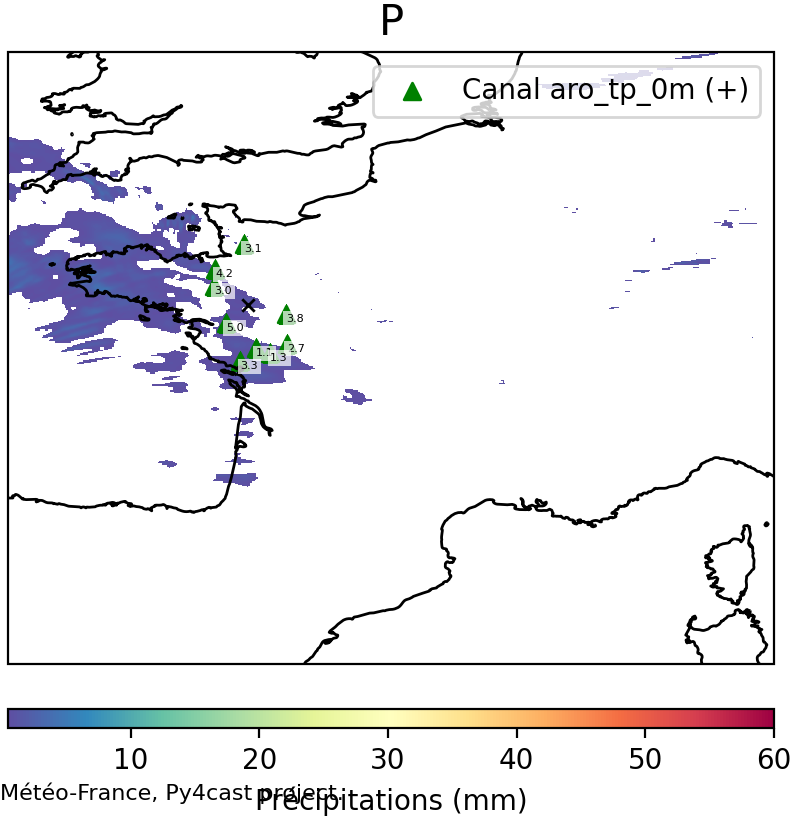
\includegraphics[width=\textwidth]{Images/titan_rain_anchors/nov-16/2023111600_feature_aro_tp_0m.png}
        \caption{Channel aro\_tp\_0m}
    \end{subfigure}
    \hfill
    \begin{subfigure}[b]{0.49\textwidth}
        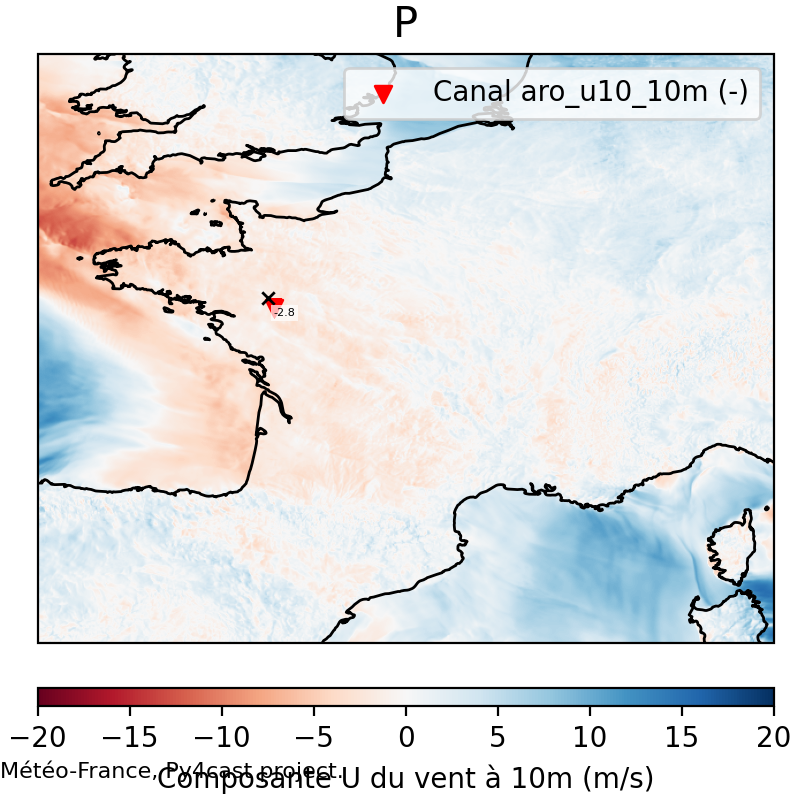
\includegraphics[width=\textwidth]{Images/titan_rain_anchors/nov-16/2023111600_feature_aro_u10_10m.png}
        \caption{Channel aro\_u10\_10m}
    \end{subfigure}
    \hfill
    \begin{subfigure}[b]{0.49\textwidth}
        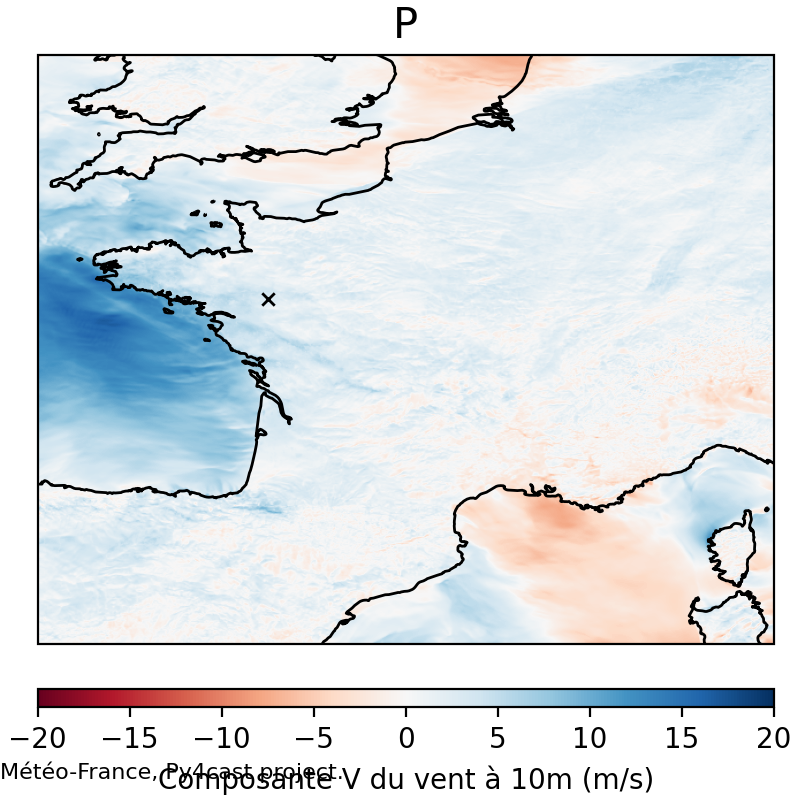
\includegraphics[width=\textwidth]{Images/titan_rain_anchors/nov-16/2023111600_feature_aro_v10_10m.png}
        \caption{Channel aro\_v10\_10m}
    \end{subfigure}
    \caption{Example of anchors applied on "rain" channels, on $16^{th}$ November data.}
    \label{fig:titan-rain-anchors-16}
\end{figure}

\begin{figure}[h]
    \centering
    \begin{subfigure}[b]{0.49\textwidth}
        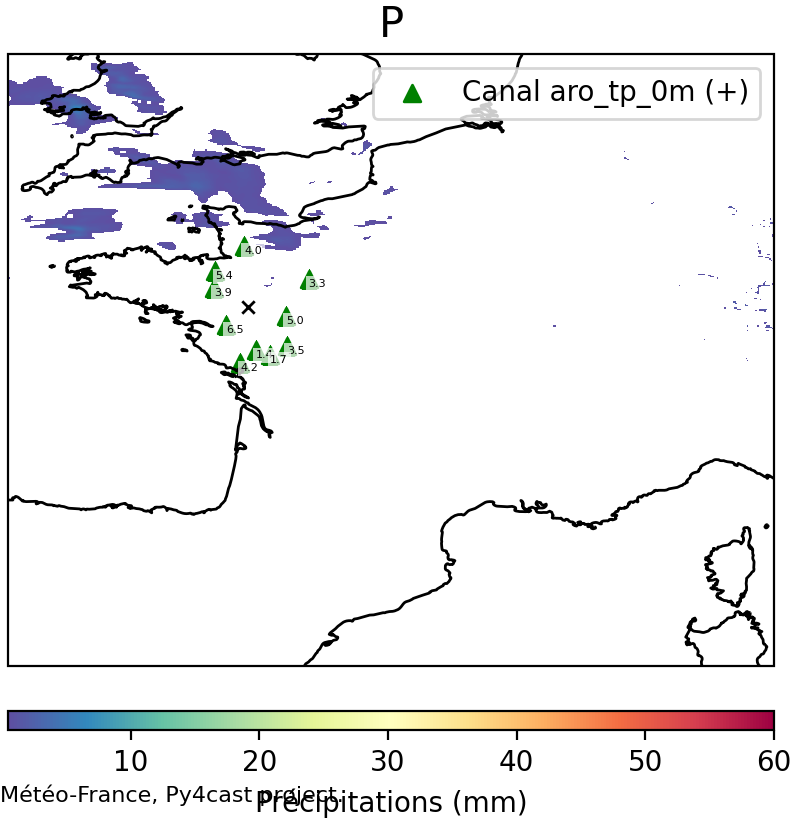
\includegraphics[width=\textwidth]{Images/titan_rain_anchors/nov-18/2023111800_feature_aro_tp_0m.png}
        \caption{Channel aro\_tp\_0m}
    \end{subfigure}
    \hfill
    \begin{subfigure}[b]{0.49\textwidth}
        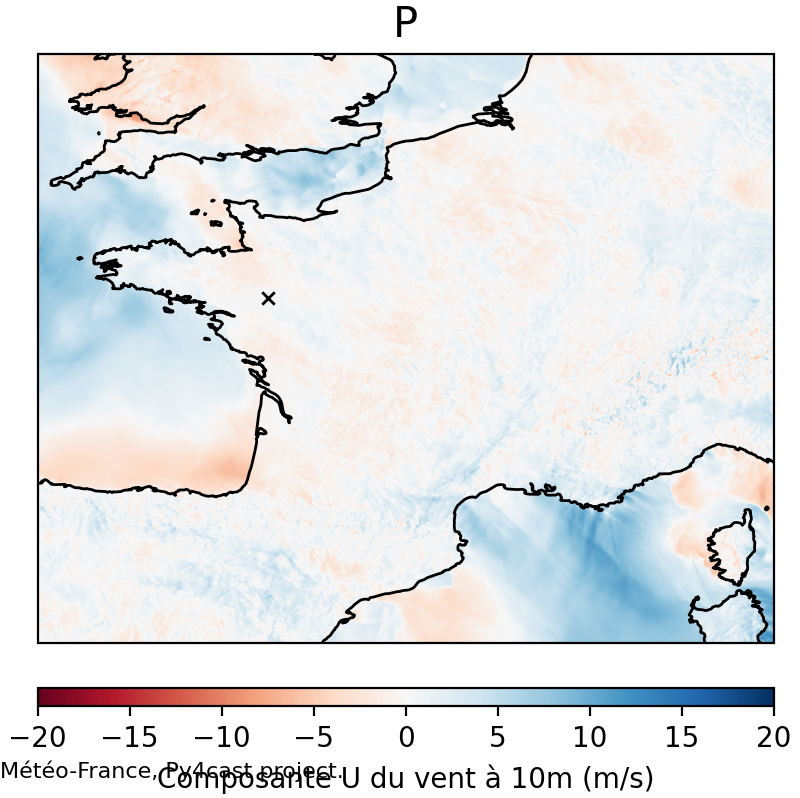
\includegraphics[width=\textwidth]{Images/titan_rain_anchors/nov-18/2023111800_feature_aro_u10_10m.png}
        \caption{Channel aro\_u10\_10m}
    \end{subfigure}
    \hfill
    \begin{subfigure}[b]{0.49\textwidth}
        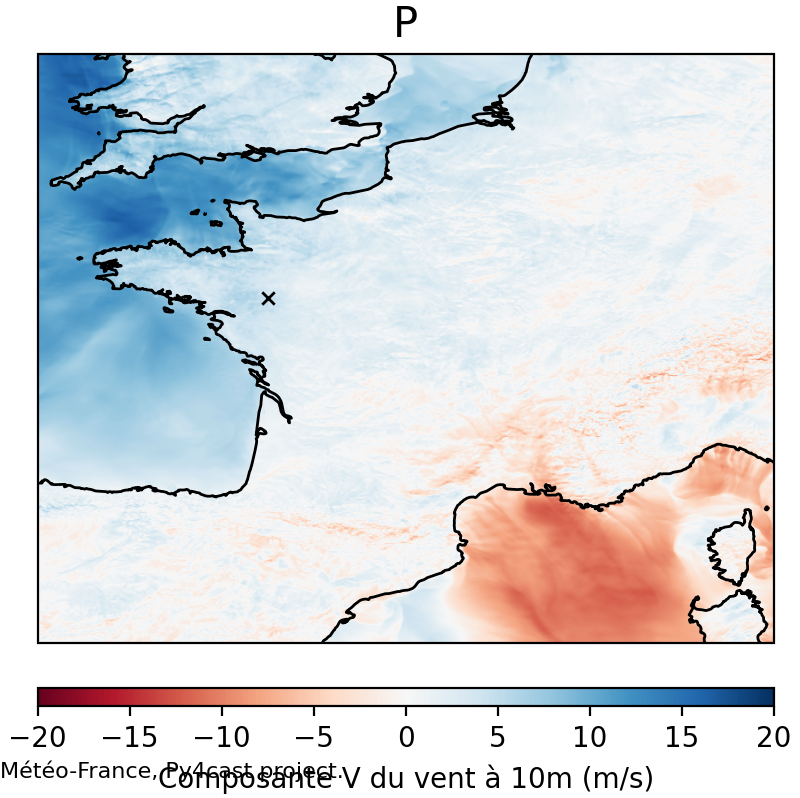
\includegraphics[width=\textwidth]{Images/titan_rain_anchors/nov-18/2023111800_feature_aro_v10_10m.png}
        \caption{Channel aro\_v10\_10m}
    \end{subfigure}
    \caption{Example of anchors applied on "rain" channels, on $18^{th}$ November data.}
    \label{fig:titan-rain-anchors-18}
\end{figure}

\begin{figure}[h]
    \centering
    \begin{subfigure}[b]{0.49\textwidth}
        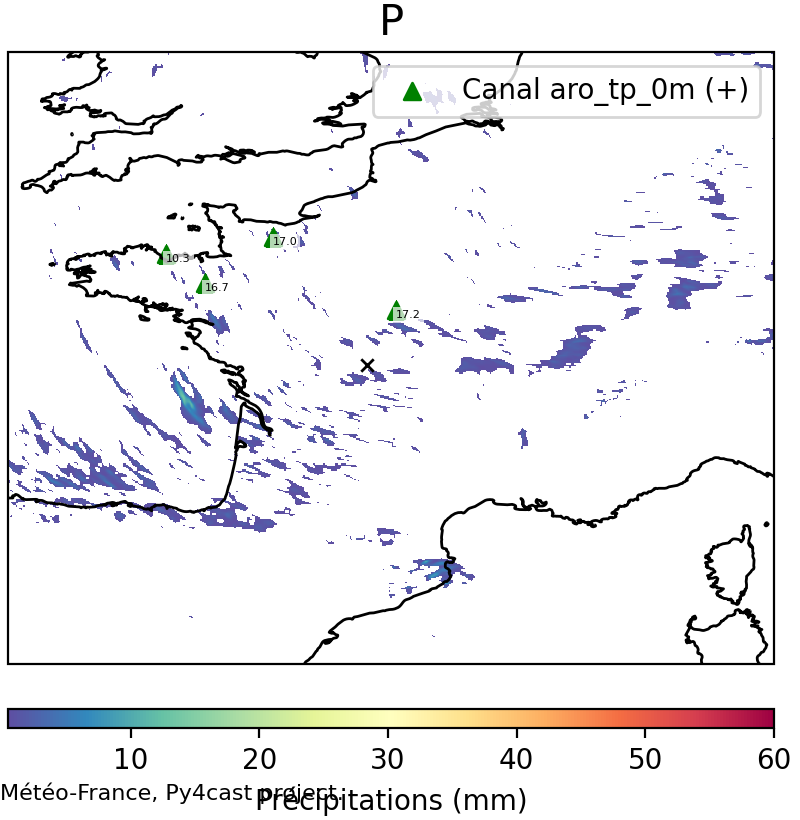
\includegraphics[width=\textwidth]{Images/titan_rain_anchors/nov-21/2023112100_feature_aro_tp_0m.png}
        \caption{Channel aro\_tp\_0m}
    \end{subfigure}
    \hfill
    \begin{subfigure}[b]{0.49\textwidth}
        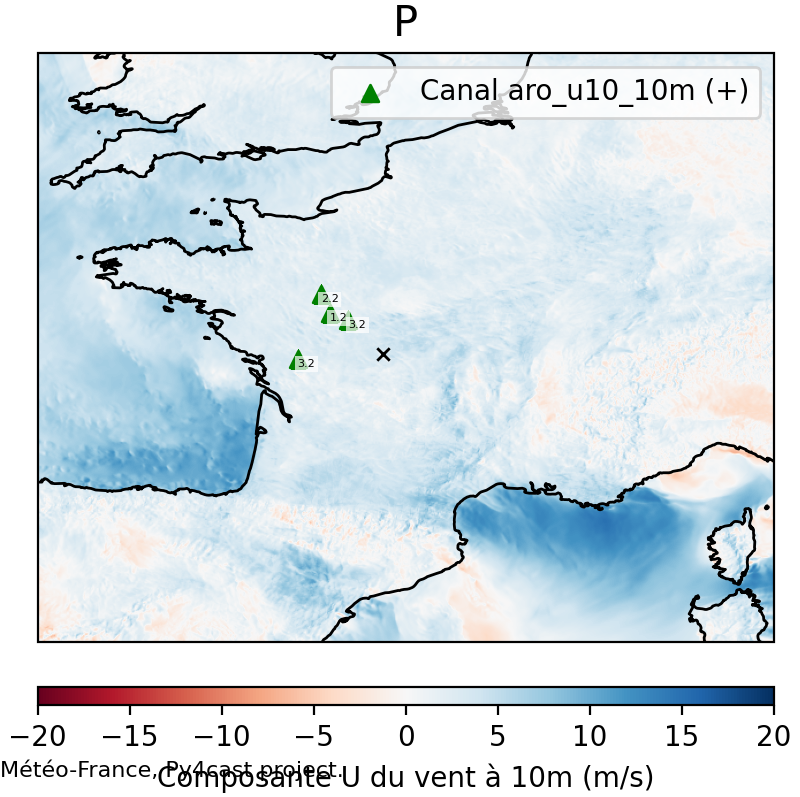
\includegraphics[width=\textwidth]{Images/titan_rain_anchors/nov-21/2023112100_feature_aro_u10_10m.png}
        \caption{Channel aro\_u10\_10m}
    \end{subfigure}
    \hfill
    \begin{subfigure}[b]{0.49\textwidth}
        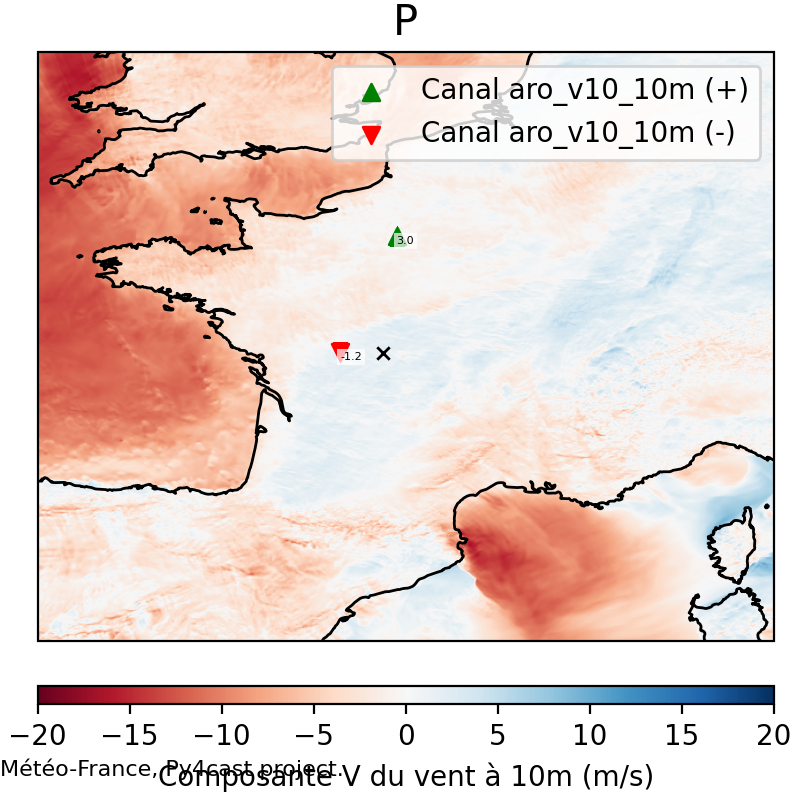
\includegraphics[width=\textwidth]{Images/titan_rain_anchors/nov-21/2023112100_feature_aro_v10_10m.png}
        \caption{Channel aro\_v10\_10m}
    \end{subfigure}
    \caption{Example of anchors applied on "rain" channels, on $21^{st}$ November data.}
    \label{fig:titan-rain-anchors-21}
\end{figure}

The results visually demonstrate how the anchors, marked by the triangle symbols on the plot, are distributed differently in each case.

The first test primarily highlights the \textit{tp\_0m} channel, showing its strong influence on the prediction for the next hour. Conversely, the lack of anchors in the wind channels indicates that no strong wind streams were influencing the region at that time.

The second test shows a scenario similar to the first. It also shows a strong influence of the \textit{tp\_0m} channel due to the approaching clouds and highlights nearby regions that would influence the target area. Additionally, we can associate the anchors in the wind channels with the stronger wind streams coming from the sea.

The third test shows some interesting insights. We chose a point in central France amidst several small concentrations of clouds. The \textit{tp\_0m} channel highlights some regions that could influence the target area, but the anchors are also well distributed across the wind channels. The anchors on the \textit{u10\_10m} and \textit{v10\_10m} channels pinpoint strategic points on the map that are likely to transport precipitation to the region.

In summary, this simplified version of the experiment demonstrates that the Anchors method can effectively describe the influential factors visible in the input images by analyzing each meteorological component.

The first key finding is that Regression Anchors successfully highlight the most influential channels for the prediction at the target location.

The second key finding is that the spatial distribution of the anchor points is coherent with the physical context of each channel and aligns with meteorological principles regarding which features would be expected to change a weather prediction in each case.


% Exportar uma lista de anchors!! para fazer uma tabela e poder analisar
\section{Discussion}
\subsection{Fairness Analysis on Tabular Data}
First if we compare the clustered PCA made with the Anchors method and with SHAP method, we can notice that the Anchors one distinguish better a region of gendered anchors.

It's significant to compare the bottom line of each Figure, that shows the filtered explanations based on high predictions and in which the 'SEX' variable in relevant to the explanation, being in the top-3 of the ranking of SHAP values or being in an anchor with a ceiling of 3 features.

So if we compare the distribution of the explanations in an Anchors approach (Figures \ref{fig:clusters_xg_tx_anchors} and \ref{fig:clusters_skrub_tx_anchors}) and SHAP approach (Figures \ref{fig:clusters_xg_tx_shap} and \ref{fig:clusters_skrub_tx_shap}), we can have more relevant insights in the Anchors one. That can be due the fact that the anchor generated by the method tests the features that are crucial to keep the prediction always the same in a local explanation, different than SHAP that gives a weight and rank the features in importance, to any feature that affects the prediction in a positive way.

For further analysis we will set the labels to reference the clusters as:
\begin{itemize}
    \item Cluster 1 - the cluster located in the bottom left of the plots
    \item Cluster 2 - the cluster located in the top of the plots
    \item Cluster 3 - the cluster located in the bottom right of the plots
\end{itemize}

Focusing on the Anchors method we can notice a concentration of gendered anchors on Clusters 1 and 2, it's important to try to understand what are the profiles of the people in each cluster, so we took the PC1 and PC2 to analyse what are the features with higher weights on each component.

\begin{table}[h]
\centering
\caption{Folktables Dataset Features}
\label{tab:folktables-pca-profiles}
\begin{tabular}{lrr}
\hline
\textbf{Feature code} & \textbf{PCA 1 (axis X)}  & \textbf{PCA 2 (axis Y)} \\
\hline
AGEP & \textbf{-0.48} & 0.24 \\
COW & -0.24 & 0.01 \\
SCHL & -0.29 & \textbf{-0.49} \\
MAR & \textbf{0.52} & -0.29 \\
OCCP & \textbf{0.31} & \textbf{0.39} \\
POBP & 0.10 & \textbf{0.51} \\
RELP & \textbf{0.45} & -0.15 \\
WKHP & -0.17 & 0.17 \\
SEX & -0.03 & \textbf{-0.30} \\
RAC1P & 0.15 & 0.26 \\
\hline
\end{tabular}
\end{table}

In the Table \ref{tab:folktables-pca-profiles} we can take the four higher values to analyse the profiles of each axis.

\begin{enumerate}
    \item PC 1 - Axis X
    \begin{enumerate}
        \item MAR (positive)
        \begin{enumerate}
            \item $\uparrow$ PC 1: means less probability of being married (MAR $> 1 \Rightarrow $ widowed, divorced, separated, never married or under 15 years old)
            \item $\downarrow$ PC 1: means more probability of being married (MAR $= 1 \Rightarrow $ married)
        \end{enumerate}

        \item AGEP (negative)
        \begin{enumerate}
            \item $\uparrow$ PC 1: means more probability of being younger
            \item $\downarrow$ PC 1: means more probability of being older
        \end{enumerate}

        \item RELP (positive)
        \begin{enumerate}
            \item $\uparrow$ PC 1: means more probability of being in a traditional family relationship at the house
            \item $\downarrow$ PC 1: means more probability of being in a different or non-traditional relashionship at the house
        \end{enumerate}

        \item OCCP (positive)
        \begin{enumerate}
            \item $\uparrow$ PC 1: means more probability of being in a high-skill, high-status occupation often requiring advanced education (e.g., management, engineering, law, medicine).
            \item $\downarrow$ PC 1: means more probability of being in a  lower-skill, manual, or service-oriented occupation that often requires less formal education or is based on on-the-job training (e.g., construction, transportation, cleaning, farming). 
        \end{enumerate}
    \end{enumerate}

    \item PC 2 - Axis Y
    \begin{enumerate}
        \item POBP (positive)
        \begin{enumerate}
            \item $\uparrow$ PC 2: means more probability of being an immigrant (higher codes are associated to people born outside of the USA)
            \item $\downarrow$ PC 2: means more probability of being a person born in the USA
        \end{enumerate}

        \item SCHL (negative)
        \begin{enumerate}
            \item $\uparrow$ PC 2: means more probability of being a person with a low level of education
            \item $\downarrow$ PC 2: means more probability of being a person with a high level of education
        \end{enumerate}

        \item OCCP (positive)
        \begin{enumerate}
            \item $\uparrow$ PC 2: means more probability of being in a high-skill, high-status occupation often requiring advanced education (e.g., management, engineering, law, medicine).
            \item $\downarrow$ PC 2: means more probability of being in a  lower-skill, manual, or service-oriented occupation that often requires less formal education or is based on on-the-job training (e.g., construction, transportation, cleaning, farming). 
        \end{enumerate}

        \item SEX (negative)
        \begin{enumerate}
            \item $\uparrow$ PC 2: means more probability of being a man (SEX $= 1 \Rightarrow $ male)
            \item $\downarrow$ PC 2: means more probability of being a woman (SEX $= 2 \Rightarrow $ female)
        \end{enumerate}
    \end{enumerate}
\end{enumerate}

Combining the clusters with the PCA analysis, we can build a profile for each cluster:

\begin{itemize}
    \item \textbf{Cluster 1: Established, Working-Class, US-born Women.} This cluster consists of older, married women born in the US, likely settled into traditional family structures and working in occupations that require less or medium formal education.
    
    \item \textbf{Cluster 2: Young, Immigrant, and Professionally Diverse Men.} This is the most diverse cluster, encompassing younger immigrant men who are not married. It includes both high-skill professionals and lower-skill laborers, representing the broad spectrum of the immigrant experience.

    \item \textbf{Cluster 3: Young, US-born, Entry-Level Service Workers.} This cluster consists of the youngest adults, born in the US, who are not married and are just starting out in the workforce, typically in low-wage, low-skill jobs with high economic vulnerability.
\end{itemize}

Seeing the generated profiles we can relate to the gendered anchors points. These points will be heavily concentrated in the bottom right-half of the plot (low PC2, which is associated with being female) and likely spread across Cluster 1 (bottom left), a part of Cluster 2 and a small female portion of Cluster 3 (bottom right).

This pattern is so common it applies to over 10\% of the population in the test set, as the coverage metric shows. That concentration can show mainly a bias between older married women and still a strong bias between immigrant women.

This type of result can lead us to think of public policies to help this population and remediate the unfairness in these specific populations.

For further proving that the Anchors really mark an area of bias we also did some tests to calculate the Disparate Impact in the area with the gendered anchors. We will use for this test the plot on the Figure \ref{fig:clusters_skrub_tx_anchors} that used the HistGradientBoosting for generating the Anchors, and that has the lowest DI between it and XGBoost.
So we selected the square around the concentrated area as shown in Figure \ref{fig:square_cluster} with coordinates $PC1 = [-2, 0]$ and $PC2 = [-2, 0]$ to calculate the DI and verify that the value is lower or similar to the DI of the whole state. In this region we have 4011 individuals, being 1300 men and 2711 women, and a DI of 0.46 with an interval of confidence of [0.44, 0.48].

\begin{figure}[h]
    \centering
    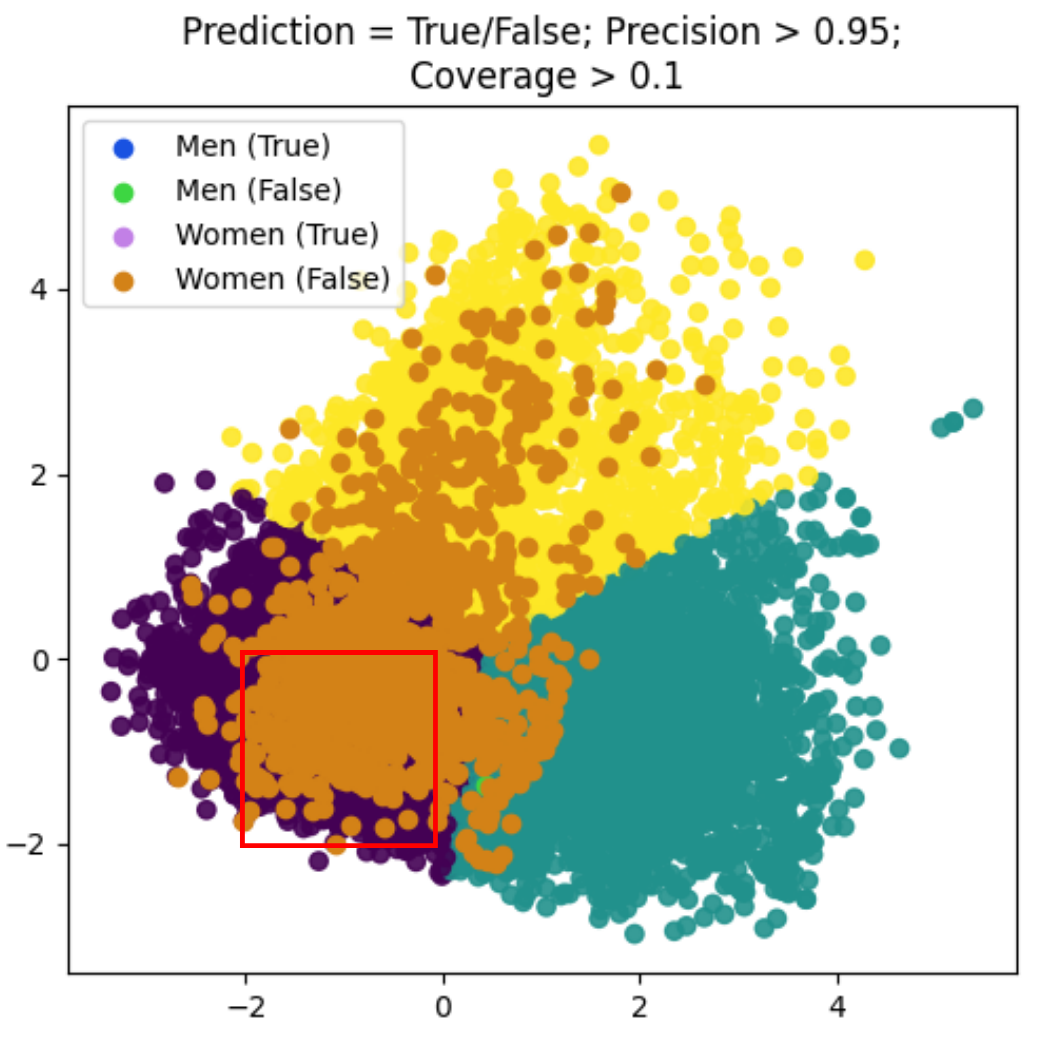
\includegraphics[width=0.7\textwidth]{Images/clustered_pca_square.png}
    \caption{Selected group of the clustered PCA in the Texas state, Model: HistGradientBoosting and XAI method: Anchors. Red square with coordinates $PC1 = [-2, 0]$ and $PC2 = [-2, 0]$}
    \label{fig:square_cluster}
\end{figure}

The DI of Texas is already very low (0.54) (Figure \ref{tab:folktables-results}), but in the region showed it can be even lower (0.46), proving that the Anchors is highligtning a region with high unfairness.

\FloatBarrier

\subsection{"Anchors Regression" applied on Multi-dimensional Data}
Having implemented our Regression Anchors approach on a simplified model with three channels, we subsequently conducted tests on other model configurations to evaluate its robustness and scalability. The configurations are described as follows:

\begin{enumerate}
\item \textbf{Rain Model (No Boundaries):} Trained exclusively on the three AROME rain channels (channels 7, 8, and 13 in Table \ref{tab:meteo_channels}), as presented in the previous results.
\item \textbf{Rain Model (With Boundaries):} Trained on the three AROME rain channels (7, 8, 13) augmented with all ARPÈGE global fields (channels 22--37) as boundary conditions.
\item \textbf{Full Model (No Boundaries):} Trained on the complete set of 21 AROME channels (1--21), without boundary conditions.
\item \textbf{Full Model (With Boundaries):} Trained on the full suite of AROME channels (1--21) combined with all ARPÈGE global fields (22--37) to provide boundary conditions.
\end{enumerate}

The following configurations were used for generating the anchors across all models:
\begin{itemize}
    \item Sampling period: November 2023.
    \item Number of counterfactuals:
    \begin{itemize}
        \item $K = 300$ for the Rain Model (lower dimensionality).
        \item $K = 2,000$ for the Full Model (higher dimensionality).
    \end{itemize}
    \item Center of target location: Centered on $(i, j)$.
    \begin{itemize}
        \item Spatial extent of the center of the perturbation mask: $\sigma_d = 150$ pixels.
    \end{itemize}
    \item Center of perturbation mask: Centered on $(\widehat{i_k}, \widehat{j_k})$.
    \begin{itemize}
        \item Spatial extent of the perturbation mask: $\sigma_e = 20$ pixels.
    \end{itemize}
    \item Prediction difference threshold: $\epsilon = 0.05$ (i.e., the prediction is considered to have changed if it varies by more than 5\%).
\end{itemize}

Focusing on a particularly illustrative case, we conducted tests on data from November $21^{st}$ for the target location $(i, j) = (300, 250)$ (near Limoges).

The results for the different models are presented in the following figures:
\begin{itemize}
\item Figure \ref{fig:titan-rain-anchors-21}: Rain Model (No Boundaries)
\item Figure \ref{fig:titan-rain-arp-anchors-21}: Rain Model (With Boundaries)
\item Figure \ref{fig:titan-full-anchors-21}: Full Model (No Boundaries)
\item Figure \ref{fig:titan-full-arp-anchors-21}: Full Model (With Boundaries)
\end{itemize}

It is important to note that the Rain Model with Boundaries did not yield satisfactory results. This is likely due to a data discrepancy: while the Rain Model is trained on lower-atmosphere AROME channels, the ARPÈGE inputs only provide atmospheric data from 250 hPa upwards. This mismatch in vertical resolution probably hindered the model's ability to integrate the boundary conditions effectively. Consequently, the following discussion will focus on the results from the Rain Model without Boundaries.

For the Full Model results, we display only the channels that contained anchors, not all 21 channels. The results for the Full Model without Boundaries can be interpreted by considering two factors: the number of anchors per channel (indicating influence) and the magnitude of their effect on the prediction.

Comparing the results of the Full Model with and without boundaries reveals that the model trained with ARPÈGE data produced more conservative explanations. It generated anchors in fewer channels and with a lower density per channel. This increased selectivity may be due to the robustness introduced by the global context provided by the ARPÈGE boundary conditions. Despite this difference, there is an intersection between the anchors found in both models (Figures \ref{fig:titan-full-arp-anchors-21} and \ref{fig:titan-full-anchors-21}), indicating agreement on the importance of certain channels and locations.

\begin{figure}[h]
    \centering
    \begin{subfigure}[b]{0.49\textwidth}
        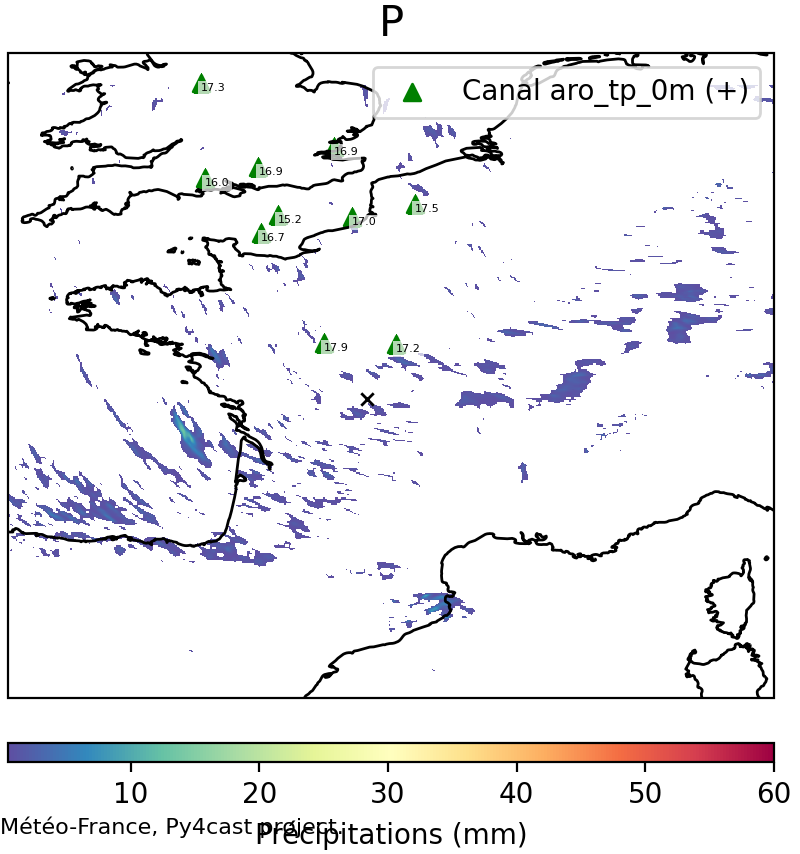
\includegraphics[width=\textwidth]{Images/titan_rain_anchors/nov-21/rain-arp/2023112100_feature_aro_tp_0m.png}
        \caption{Channel aro\_tp\_0m}
    \end{subfigure}
    \hfill
    \begin{subfigure}[b]{0.49\textwidth}
        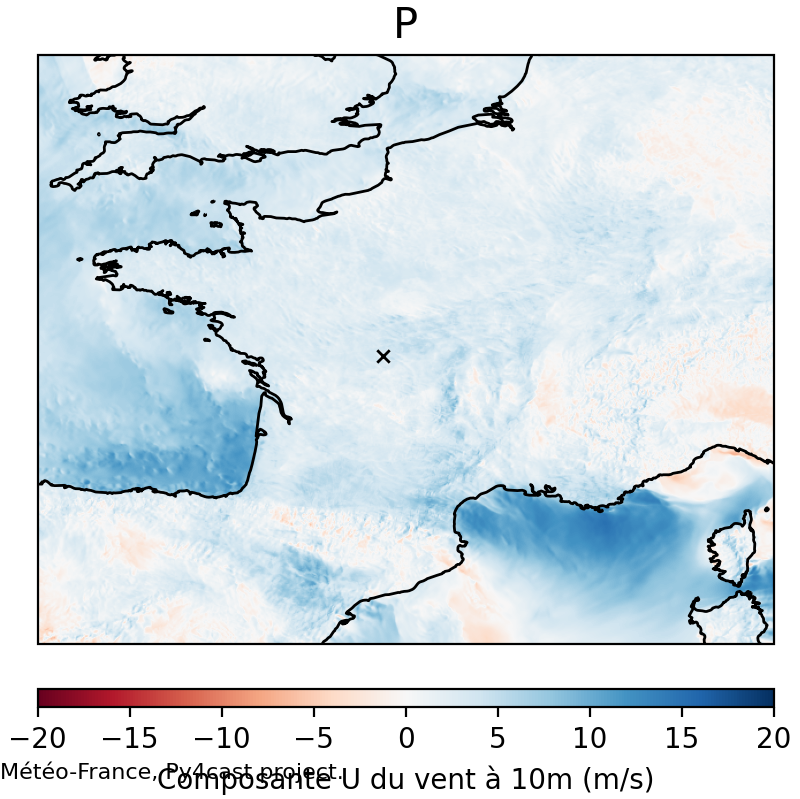
\includegraphics[width=\textwidth]{Images/titan_rain_anchors/nov-21/rain-arp/2023112100_feature_aro_u10_10m.png}
        \caption{Channel aro\_u10\_10m}
    \end{subfigure}
    \hfill
    \begin{subfigure}[b]{0.49\textwidth}
        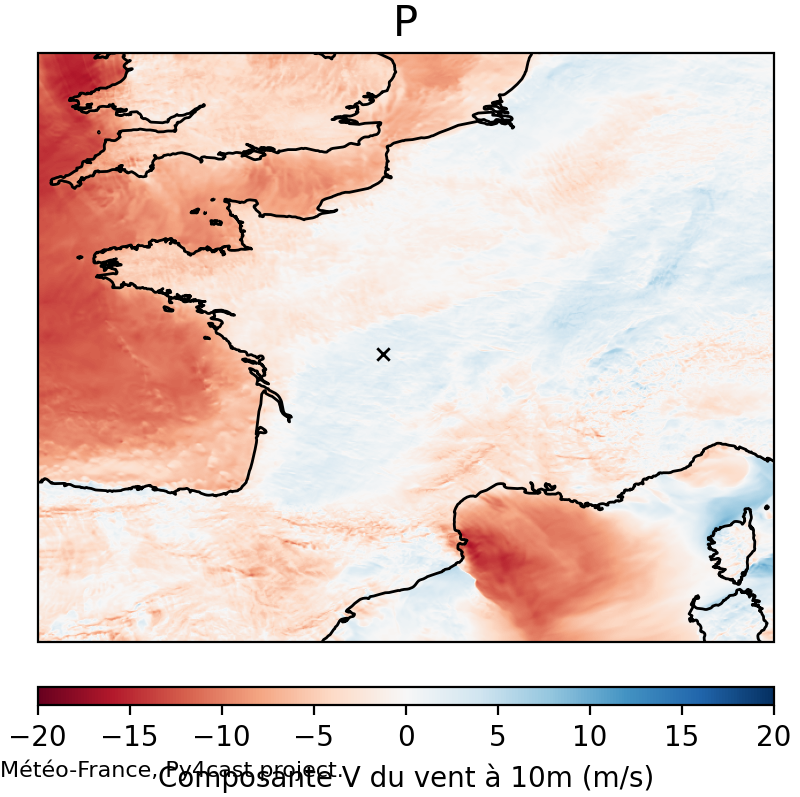
\includegraphics[width=\textwidth]{Images/titan_rain_anchors/nov-21/rain-arp/2023112100_feature_aro_v10_10m.png}
        \caption{Channel aro\_v10\_10m}
    \end{subfigure}
    \caption{Example of anchors applied on Rain Model (With Boundaries), on $21^{st}$ November data.}
    \label{fig:titan-rain-arp-anchors-21}
\end{figure}

\begin{figure}[h]
    \centering
    \begin{subfigure}[b]{0.44\textwidth}
        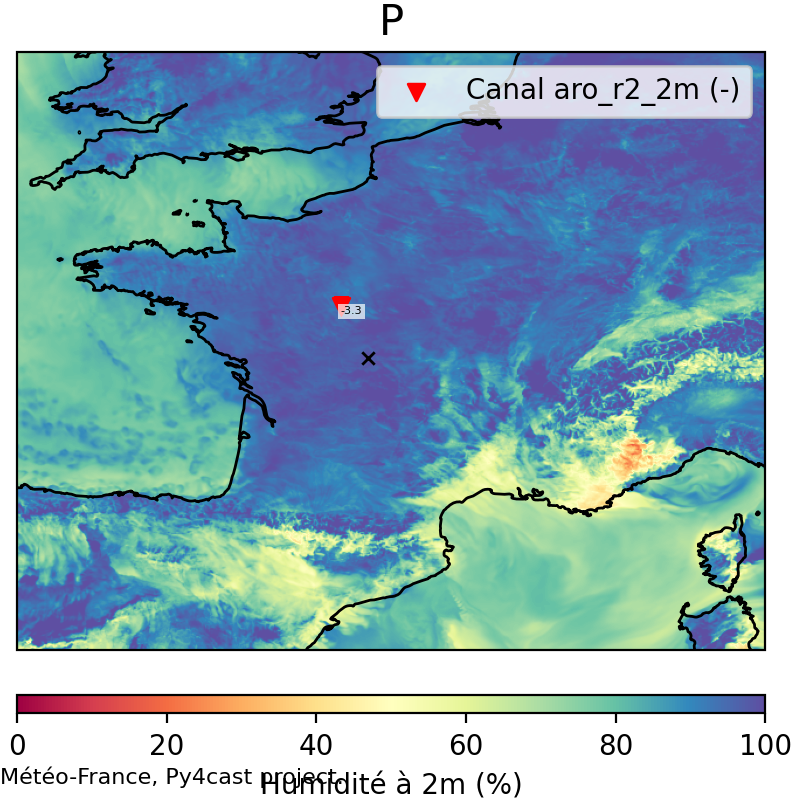
\includegraphics[width=\textwidth]{Images/titan_rain_anchors/nov-21/complete/2023112100_feature_aro_r2_2m.png}
        \caption{Channel aro\_r2\_2m}
    \end{subfigure}
    \hfill
    \begin{subfigure}[b]{0.44\textwidth}
        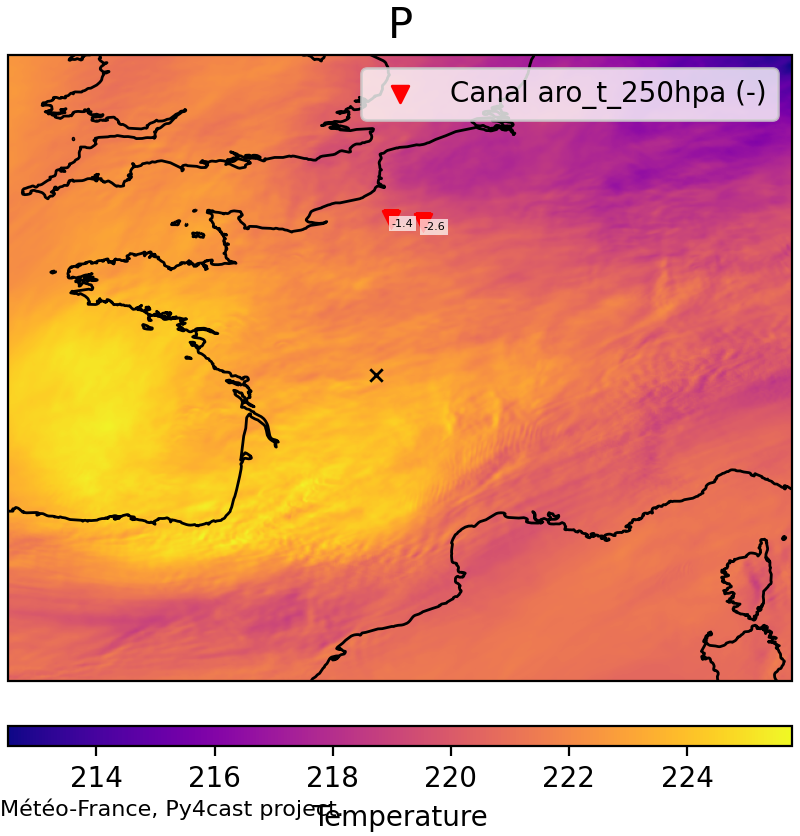
\includegraphics[width=\textwidth]{Images/titan_rain_anchors/nov-21/complete/2023112100_feature_aro_t_250hpa.png}
        \caption{Channel aro\_t\_250hpa}
    \end{subfigure}
    \hfill
    \begin{subfigure}[b]{0.44\textwidth}
        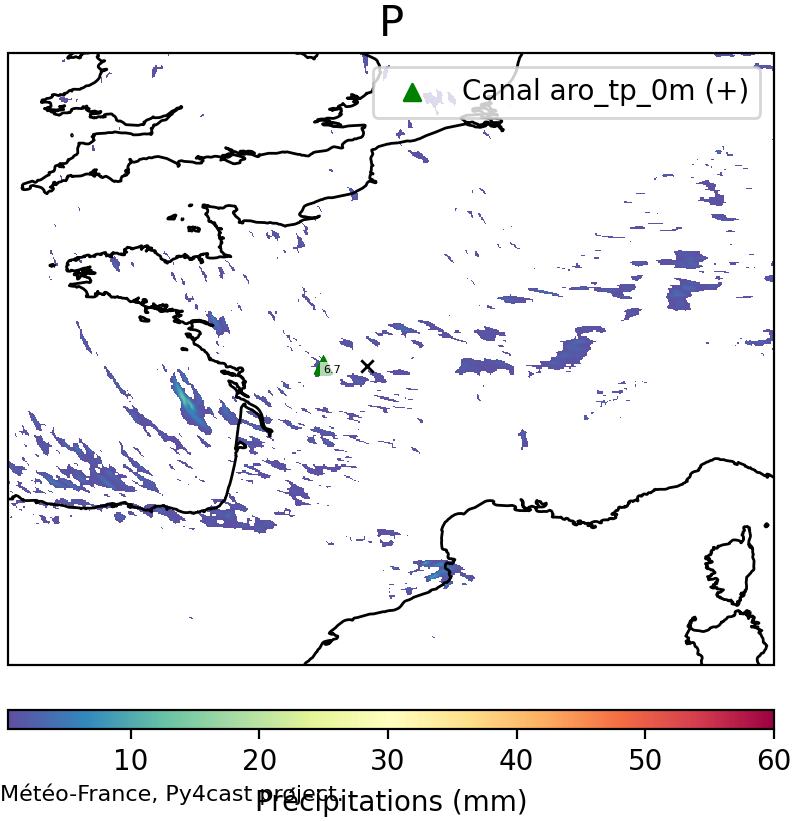
\includegraphics[width=\textwidth]{Images/titan_rain_anchors/nov-21/complete/2023112100_feature_aro_tp_0m.png}
        \caption{Channel aro\_tp\_0m}
    \end{subfigure}
    \hfill
    \begin{subfigure}[b]{0.44\textwidth}
        \includegraphics[width=\textwidth]{Images/titan_rain_anchors/nov-21/complete/2023112100_feature_aro_u_250hpa.png}
        \caption{Channel aro\_u\_250hpa}
    \end{subfigure}
    \hfill
    \begin{subfigure}[b]{0.44\textwidth}
        \includegraphics[width=\textwidth]{Images/titan_rain_anchors/nov-21/complete/2023112100_feature_aro_u_500hpa.png}
        \caption{Channel aro\_u\_500hpa}
    \end{subfigure}
    \hfill
    \begin{subfigure}[b]{0.44\textwidth}
        \includegraphics[width=\textwidth]{Images/titan_rain_anchors/nov-21/complete/2023112100_feature_aro_v_250hpa.png}
        \caption{Channel aro\_v\_250hpa}
    \end{subfigure}
    \caption{Anchors applied on Full Model (No Boundaries), on $21^{st}$ November data. (Part 1)}
\end{figure}

\begin{figure}[h]
    \ContinuedFloat
    \begin{subfigure}[b]{0.44\textwidth}
        \includegraphics[width=\textwidth]{Images/titan_rain_anchors/nov-21/complete/2023112100_feature_aro_z_250hpa.png}
        \caption{Channel aro\_z\_250hpa}
    \end{subfigure}
    \hfill
    \begin{subfigure}[b]{0.44\textwidth}
        \includegraphics[width=\textwidth]{Images/titan_rain_anchors/nov-21/complete/2023112100_feature_aro_z_500hpa.png}
        \caption{Channel aro\_z\_500hpa}
    \end{subfigure}
    \hfill
    \begin{subfigure}[b]{0.44\textwidth}
        \includegraphics[width=\textwidth]{Images/titan_rain_anchors/nov-21/complete/2023112100_feature_aro_z_700hpa.png}
        \caption{Channel aro\_z\_700hpa}
    \end{subfigure}
    \hfill
    \begin{subfigure}[b]{0.44\textwidth}
        \includegraphics[width=\textwidth]{Images/titan_rain_anchors/nov-21/complete/2023112100_feature_aro_z_850hpa.png}
        \caption{Channel aro\_z\_850hpa}
    \end{subfigure}
    \caption{Anchors applied on Full Model (No Boundaries), on $21^{st}$ November data. (Part 2)}
    \label{fig:titan-full-anchors-21}
\end{figure}

  
\begin{figure}[h]
    \centering
    \begin{subfigure}[b]{0.49\textwidth}
        \includegraphics[width=\textwidth]{Images/titan_rain_anchors/nov-21/complete-arp/2023112100_feature_aro_tp_0m.png}
        \caption{Channel aro\_tp\_0m}
    \end{subfigure}
    \hfill
    \begin{subfigure}[b]{0.49\textwidth}
        \includegraphics[width=\textwidth]{Images/titan_rain_anchors/nov-21/complete-arp/2023112100_feature_aro_z_500hpa.png}
        \caption{Channel aro\_z\_500hpa}
    \end{subfigure}
    \hfill
    \begin{subfigure}[b]{0.49\textwidth}
        \includegraphics[width=\textwidth]{Images/titan_rain_anchors/nov-21/complete-arp/2023112100_feature_aro_z_700hpa.png}
        \caption{Channel aro\_z\_700hpa}
    \end{subfigure}
    \caption{Anchors applied on Full Model (With Boundaries), on $21^{st}$ November data. (Part 1)}
    \label{fig:titan-full-arp-anchors-21}
\end{figure}

\subsection{"Anchors Regression" applied on LLM}
The application of the "Regression Anchors" method to high-dimensional, spatial-temporal data, as demonstrated in weather forecasting, establishes a versatile framework that can be adapted to other complex domains. A direct and promising extension would be to LLMs.

The core methodology remains applicable: one would define a precise prediction to explain (e.g., a model's sentiment score or its choice of a specific token) and generate counterfactuals by perturbing the input. The concept of a spatial perturbation mask would be translated into a textual mask, where certain words or tokens in a sentence are perturbed or replaced according to a defined strategy. The precision and coverage metrics would then identify the minimal set of words (the "anchor") that most reliably controls the model's output.

While the exciting prospect of applying this methodology to LLMs was beyond the scope of this internship due to time constraints, it represents a logical and valuable progression for this research, bridging explainability between perceptual (vision/weather) and semantic (language) AI systems.
\section{Conclusion}
This work explored the application of the Anchors XAI method across two distinct domains: tabular data for fairness auditing and high-dimensional spatial data for weather forecasting. The results demonstrate that Anchors possesses a unique capability to provide focused, direct, and actionable insights, regardless of the data's complexity.

In the tabular domain with the Folktables dataset, Anchors proved to be a powerful tool for identifying specific vulnerabilities and biases within model predictions. By generating high-precision rules, it pinpointed the exact demographic and socioeconomic factors that led to discriminatory outcomes, such as systematically lower income predictions for certain groups. This granular understanding is the first crucial step toward designing targeted bias mitigation strategies, moving beyond simply detecting bias to explaining its precise mechanisms.

When applied to the high-dimensionality of meteorological data, Anchors revealed its versatility. The method transitioned from auditing model fairness to auditing model reasoning in a physical context. It successfully identified not just if a prediction was made, but which specific areas and meteorological variables were most influential for that prediction. This transforms Anchors into a powerful tool for regional influence analysis, allowing meteorologists to understand which upstream regions have the greatest impact on a local forecast.

Furthermore, the method demonstrated potential for proactive vulnerability mapping. By highlighting surrounding areas that significantly influence a target location, Anchors can reveal geographic points of failure or sensitivity. This is invaluable for planning and preparedness, as it allows us to identify zones where extreme weather events elsewhere could have a critical downstream impact, thereby improving risk assessment and resource allocation.

In conclusion, from auditing societal biases in algorithms to diagnosing the physical drivers of weather models, the Anchors method has proven to be exceptionally adept at providing focused explanations. It moves past global model interpretation to deliver local, instance-based insights that are directly applicable to solving real-world problems, whether they pertain to social justice or natural phenomena. This work establishes a robust foundation for using explainability not just as a diagnostic tool, but as a guide for actionable intervention in both technical and societal systems.

{
\cleardoublepage % coloca o número de página correto das referências bibliográficas no sumário
\phantomsection % faz o link para a página correta das referências bibliográficas
\addcontentsline{}{section}{References}
\bibliography{bib}
}

\appendix
\section{Apendix Title}
\label{ap:Opt}

\begin{figure}[h]
    \centering
    \begin{subfigure}[b]{0.48\textwidth}
        \includegraphics[width=\textwidth]{Images/curve_roc_folktables/roc_curve_TX_lr.png}
        \caption{Curve ROC (AUC = 0.848): model = Logistic Regression}
        \label{fig:TX_lr}
    \end{subfigure}
    \hfill
    \begin{subfigure}[b]{0.48\textwidth}
        \includegraphics[width=\textwidth]{Images/curve_roc_folktables/roc_curve_TX_NN.png}
        \caption{Curve ROC (AUC = 0.795): model = Neural Network}
        \label{fig:TX_nn}
    \end{subfigure}

    \begin{subfigure}[b]{0.48\textwidth}
        \includegraphics[width=\textwidth]{Images/curve_roc_folktables/roc_curve_TX_xgb.png}
        \caption{Curve ROC (AUC = 0.883): model = XGBoost}
        \label{fig:TX_xgb}
    \end{subfigure}
    \hfill
    \begin{subfigure}[b]{0.48\textwidth}
        \includegraphics[width=\textwidth]{Images/curve_roc_folktables/roc_curve_TX_skrub.png}
        \caption{Curve ROC (AUC = 0.886): model = HistGradientBoosting}
        \label{fig:TX_skrub}
    \end{subfigure}
    \caption{Comparison of the models trained on the sub dataset of the Texas state}
    \label{fig:roc_tx}
\end{figure}

\begin{figure}[h]
    \centering
    \begin{subfigure}[b]{0.9\textwidth}
        \includegraphics[width=\textwidth]{Images/pca/pca_xg_ca_anchors.png}
        \caption{Model: XGBoost, XAI method: Anchors}
        \label{fig:pca_xg_ca_anchors}
    \end{subfigure}
    \hfill
    \begin{subfigure}[b]{0.9\textwidth}
        \includegraphics[width=\textwidth]{Images/pca/pca_skrub_ca_anchors.png}
        \caption{Model: HistGradientBoosting, XAI method: Anchors}
        \label{fig:pca_skrub_ca_anchors}
    \end{subfigure}
    \caption{PCA of the test dataset in the California state (Part 1)}
 \end{figure}

\begin{figure}[h]
    \ContinuedFloat
    \begin{subfigure}[b]{0.9\textwidth}
        \includegraphics[width=\textwidth]{Images/pca/pca_xg_ca_shap.png}
        \caption{Model: XGBoost, XAI method: SHAP}
        \label{fig:pca_xg_ca_shap}
    \end{subfigure}
    \hfill
    \begin{subfigure}[b]{0.9\textwidth}
        \includegraphics[width=\textwidth]{Images/pca/pca_skrub_ca_shap.png}
        \caption{Model: HistGradientBoosting, XAI method: SHAP}
        \label{fig:pca_skrub_ca_shap}
    \end{subfigure}
    \caption{PCA of the test dataset in the California state (Part 2)}
    \label{fig:pca_ca}
\end{figure}
    


\begin{figure}[h]
    \centering
    \begin{subfigure}[b]{0.9\textwidth}
        \includegraphics[width=\textwidth]{Images/pca/pca_xg_ny_anchors.png}
        \caption{Model: XGBoost, XAI method: Anchors}
        \label{fig:pca_xg_ny_anchors}
    \end{subfigure}
    \hfill
    \begin{subfigure}[b]{0.9\textwidth}
        \includegraphics[width=\textwidth]{Images/pca/pca_skrub_ny_anchors.png}
        \caption{Model: HistGradientBoosting, XAI method: Anchors}
        \label{fig:pca_skrub_ny_anchors}
    \end{subfigure}
\caption{PCA of the test dataset in the New York state (Part 1)}
 \end{figure}

\begin{figure}[h]
    \ContinuedFloat
    \begin{subfigure}[b]{0.9\textwidth}
        \includegraphics[width=\textwidth]{Images/pca/pca_xg_ny_shap.png}
        \caption{Model: XGBoost, XAI method: SHAP}
        \label{fig:pca_xg_ny_shap}
    \end{subfigure}
    \hfill
    \begin{subfigure}[b]{0.9\textwidth}
        \includegraphics[width=\textwidth]{Images/pca/pca_skrub_ny_shap.png}
        \caption{Model: HistGradientBoosting, XAI method: SHAP}
        \label{fig:pca_skrub_ny_shap}
    \end{subfigure}
    \caption{PCA of the test dataset in the New York state (Part 2)}
    \label{fig:pca_ny}
\end{figure}

\begin{figure}[h]
    \centering
    \begin{subfigure}[b]{0.9\textwidth}
        \includegraphics[width=\textwidth]{Images/distribution_folktables/pca_xg_ca_anchors.png}
        \caption{Model: XGBoost, XAI method: Anchors}
        \label{fig:distr_xg_ca_anchors}
    \end{subfigure}
    \hfill
    \begin{subfigure}[b]{0.9\textwidth}
        \includegraphics[width=\textwidth]{Images/distribution_folktables/pca_skrub_ca_anchors.png}
        \caption{Model: HistGradientBoosting, XAI method: Anchors}
        \label{fig:distr_skrub_ca_anchors}
    \end{subfigure}
    \caption{Comparison of the gendered explanations between True and False predictions in the California state (Part 1)}
 \end{figure}

\begin{figure}[h]
    \ContinuedFloat
    \begin{subfigure}[b]{0.9\textwidth}
        \includegraphics[width=\textwidth]{Images/distribution_folktables/pca_xg_ca_shap.png}
        \caption{Model: XGBoost, XAI method: SHAP}
        \label{fig:distr_xg_ca_shap}
    \end{subfigure}
    \hfill
    \begin{subfigure}[b]{0.9\textwidth}
        \includegraphics[width=\textwidth]{Images/distribution_folktables/pca_skrub_ca_shap.png}
        \caption{Model: HistGradientBoosting, XAI method: SHAP}
        \label{fig:distr_skrub_ca_shap}
    \end{subfigure}
    \caption{Comparison of the gendered explanations between True and False predictions in the California state (Part 2)}
    \label{fig:distr_ca}
\end{figure}

\begin{figure}[h]
    \centering
    \begin{subfigure}[b]{0.9\textwidth}
        \includegraphics[width=\textwidth]{Images/distribution_folktables/pca_xg_ny_anchors.png}
        \caption{Model: XGBoost, XAI method: Anchors}
        \label{fig:distr_xg_ny_anchors}
    \end{subfigure}
    \hfill
    \begin{subfigure}[b]{0.9\textwidth}
        \includegraphics[width=\textwidth]{Images/distribution_folktables/pca_skrub_ny_anchors.png}
        \caption{Model: HistGradientBoosting, XAI method: Anchors}
        \label{fig:distr_skrub_ny_anchors}
    \end{subfigure}
    \caption{Comparison of the gendered explanations between True and False predictions in the New York state (Part 1)}
 \end{figure}

\begin{figure}[h]
    \ContinuedFloat
    \begin{subfigure}[b]{0.9\textwidth}
        \includegraphics[width=\textwidth]{Images/distribution_folktables/pca_xg_ny_shap.png}
        \caption{Model: XGBoost, XAI method: SHAP}
        \label{fig:distr_xg_ny_shap}
    \end{subfigure}
    \hfill
    \begin{subfigure}[b]{0.9\textwidth}
        \includegraphics[width=\textwidth]{Images/distribution_folktables/pca_skrub_ny_shap.png}
        \caption{Model: HistGradientBoosting, XAI method: SHAP}
        \label{fig:distr_skrub_ny_shap}
    \end{subfigure}
    \caption{Comparison of the gendered explanations between True and False predictions in the New York state (Part 2)}
    \label{fig:distr_ny}
\end{figure}

\begin{figure}[h]
    \centering
    \begin{subfigure}[b]{1.0\textwidth}
        \includegraphics[width=\textwidth]{Images/clustered_pca/clusters_xg_tx_anchors.png}
        \caption{Model: XGBoost, XAI method: Anchors}
        \label{fig:clusters_xg_tx_anchors}
    \end{subfigure}

    \begin{subfigure}[b]{1.0\textwidth}
        \includegraphics[width=\textwidth]{Images/clustered_pca/clusters_skrub_tx_anchors.png}
        \caption{Model: HistGradientBoosting, XAI method: Anchors}
        \label{fig:clusters_skrub_tx_anchors}
    \end{subfigure}
    \caption{Comparison of the clustered PCA in the Texas state, putting in evidence gendered explanations (Part 1)}
\end{figure}

\begin{figure}[h]
    \ContinuedFloat
    \begin{subfigure}[b]{1.0\textwidth}
        \includegraphics[width=\textwidth]{Images/clustered_pca/clusters_xg_tx_shap.png}
        \caption{Model: XGBoost, XAI method: SHAP}
        \label{fig:clusters_xg_tx_shap}
    \end{subfigure}

    \begin{subfigure}[b]{1.0\textwidth}
        \includegraphics[width=\textwidth]{Images/clustered_pca/clusters_skrub_tx_shap.png}
        \caption{Model: HistGradientBoosting, XAI method: SHAP}
        \label{fig:clusters_skrub_tx_shap}
    \end{subfigure}

    \caption{Comparison of the clustered PCA in the Texas state, putting in evidence gendered explanations (Part 2)}
    \label{fig:clusters_tx}
\end{figure}

\end{document}
